% ICML 2025 Paper Template for Overleaf
% Auto-generated by Anonymous Research Pipeline - Phase 6.5.1
%
% Instructions:
% 1. Upload this folder to Overleaf
% 2. Ensure icml2025.sty is in the same directory
% 3. Compile with pdfLaTeX
%
\documentclass{article}

% ICML 2025 style - download from https://icml.cc/Conferences/2025/StyleAuthorInstructions
% \usepackage{icml2025}  % Uncomment when icml2025.sty is available (Overleaf)

% Standard packages
\usepackage{microtype}
\usepackage{graphicx}
\usepackage{booktabs}
\usepackage{hyperref}
\usepackage{amsmath}
\usepackage{amssymb}

% For better table formatting
\usepackage{multirow}
\usepackage{makecell}

% Bibliography
\usepackage{natbib}

% Fallback title/author (used when icml2025.sty not available)
\title{When Adversarial Examples Improve Calibration:\\
Construction-Method-Dependent Calibration Degradation in Open-Weight LLMs}
\author{Anonymous Author \\ Anonymous Institution}
\date{2026-08-25}

% ============================================================================
% DOCUMENT METADATA
% ============================================================================

\begin{document}

\maketitle

% ============================================================================
% ABSTRACT
% ============================================================================

\begin{abstract}
When we evaluated an open-weight LLM on model-in-the-loop adversarial NLP benchmarks (ANLI), we found a counterintuitive result: calibration \textit{improved} relative to the clean baseline ($\Delta$ECE $= -0.041$ for ANLI R1). The adversarial benchmark, designed to expose model failures, made the model appear better calibrated. Yet human-adversarially crafted NLI examples (AdvGLUE MNLI) produced the opposite --- a 7.1 percentage-point ECE increase ($\Delta$ECE $= +0.071$). Calibration robustness under adversarial conditions is not universal: it depends critically on \textit{how} adversarial examples were constructed. We measure Expected Calibration Error (ECE) directly on adversarial NLP benchmark splits for an open-weight LLM (Llama-2-7b-hf), finding that calibration degradation is conditional on adversarial construction method and task type. RLHF alignment moderates this pattern in a benchmark-type-dependent manner --- consistently improving calibration robustness on model-in-loop adversarial conditions (100\% moderation rate across all ANLI rounds) while exacerbating degradation on static human-adversarial benchmarks (alignment tax: $\Delta\Delta$ECE $= -0.026$ on AdvGLUE). In this single-model pilot study, these findings motivate adversarial calibration measurement as a distinct research problem from adversarial accuracy robustness, and provide a conditional framework --- construction method $\times$ task type $\times$ RLHF alignment --- for understanding when and how adversarial perturbation may degrade model reliability signals in deployment.

\end{abstract}

% ============================================================================
% MAIN CONTENT
% ============================================================================

\section{Introduction}

When we evaluated an open-weight language model on the ANLI R1 benchmark --- a dataset specifically constructed so that human annotators could fool state-of-the-art NLP models --- we found that the model's Expected Calibration Error \textit{decreased} relative to its performance on clean MultiNLI. The adversarial benchmark, designed to expose model failures, made the model appear \textit{better calibrated}. This result was not an error. It reveals a fundamental property of how adversarial construction methods interact with model confidence: in a model-in-the-loop adversarial benchmark, the examples are selected precisely because the model fails on them --- and a model that fails with appropriately low confidence is, by definition, well-calibrated.

This observation motivates the central question of our work: \textbf{does adversarial perturbation of NLP benchmarks actually degrade LLM calibration, and if so, under what conditions?}

\subsection{The Problem}

Calibration --- the alignment between predicted confidence and observed accuracy --- is a critical reliability property for deployed language models. A model that assigns 90\% confidence to its predictions should be correct 90\% of the time; deviations from this correspondence make model confidence unreliable as a safety signal. The field has developed robust measurement tools, most notably Expected Calibration Error (ECE) \citep{guo2017calibration}, and has documented that modern neural networks are systematically overconfident under distribution shift \citep{minderer2021revisiting}.

At the same time, adversarial NLP benchmarks --- AdvGLUE \citep{wang2021adversarial} and ANLI \citep{nie2020adversarial} --- have become standard for evaluating LLM robustness under distribution shift, typically reporting accuracy degradation. But accuracy degradation alone does not characterize the reliability of model confidence under adversarial conditions. A model that becomes \textit{less} accurate but \textit{proportionally less confident} may be better calibrated than one that maintains confidence while failing more often.

The deeper problem is that adversarial benchmarks are not a single category. AdvGLUE uses \textit{human adversaries} who craft perturbations to fool existing models; ANLI uses a \textit{model-in-the-loop} construction where examples are selected by human annotators specifically when they cause model errors. These construction methods produce qualitatively different distributions of model behavior --- and consequently, different calibration effects. Yet prior calibration studies treat adversarial perturbation as a monolithic distribution shift, analogous to the vision-domain corruptions studied by \citet{minderer2021revisiting}. Whether this analogy holds in NLP, and whether RLHF alignment moderates the effect, has not been tested.

\textbf{The gap:} No published work measures logit-based ECE on adversarial NLP benchmark splits (AdvGLUE, ANLI) for open-weight LLMs, or examines how adversarial construction method and RLHF alignment jointly determine calibration outcomes under adversarial conditions.

\subsection{Key Insight}

Our central finding is that adversarial calibration degradation in LLMs is \textbf{task-type and construction-method conditional}, not universal. Human-adversarial NLI examples (AdvGLUE MNLI) produce reliable calibration degradation: $\Delta$ECE $= +0.071$, a 7.1 percentage-point increase in Expected Calibration Error relative to clean MultiNLI. Model-in-the-loop adversarial NLI examples (ANLI R1/R2) produce calibration \textit{improvement}: $\Delta$ECE $= -0.041$ for R1. Binary classification tasks (QQP, SST-2) show reversed $\Delta$ECE regardless of adversarial method. And RLHF alignment conditionally moderates these effects --- helping for model-in-loop adversarial (100\% moderation rate across ANLI rounds) but exacerbating calibration degradation for static human-adversarial benchmarks ($\Delta\Delta$ECE $= -0.026$, chat worse than base on AdvGLUE).

The resolution to the opening paradox follows directly: in model-in-the-loop adversarial benchmarks, examples are selected to cause errors; a model that fails with appropriately moderate confidence on such examples is demonstrating calibration, not miscalibration. Human-adversarial examples, by contrast, exploit surface features to trigger high confidence on wrong answers --- the classic miscalibration mechanism.

\subsection{Contributions}

Our investigation of adversarial LLM calibration yields three contributions that build from existence to mechanism to conditionality:

\textbf{(1) First measurement of logit-based ECE on adversarial NLP benchmarks.} We measure ECE directly on AdvGLUE and ANLI benchmark splits for Llama-2-7b-hf, establishing $\Delta$ECE as a measurable, meaningful quantity for adversarial calibration stress testing. This fills the gap between adversarial robustness evaluation (accuracy-only) and calibration measurement (clean-data-only). Our JSONL logit caching strategy enables multiple downstream calibration analyses (label preservation, confidence-accuracy decoupling, per-cell $\Delta$ECE, RLHF comparison) from a single inference pass, making multi-cell adversarial calibration analysis computationally feasible.

\textbf{(2) Evidence that calibration degradation is task-type and construction-method conditional.} Human-adversarial NLI examples (AdvGLUE MNLI: $\Delta$ECE $= +0.071$) produce calibration degradation; model-in-the-loop adversarial examples (ANLI R1/R2: $\Delta$ECE $< 0$) produce calibration improvement; and the ANLI difficulty gradient (R1 $\rightarrow$ R2 $\rightarrow$ R3) shows a smooth transition from improvement to degradation as adversarial difficulty increases. Binary classification tasks consistently show reversed $\Delta$ECE. This nuances the vision-domain finding that distribution shift uniformly degrades calibration.

\textbf{(3) Evidence that RLHF alignment conditionally moderates adversarial calibration degradation.} We compare Llama-2-7b-hf (base) and Llama-2-7b-chat across ANLI and AdvGLUE conditions. RLHF moderation is confirmed for model-in-loop adversarial (100\% of ANLI rounds show $\Delta\Delta$ECE $> 0.01$ favoring chat), but reversed for static human-adversarial benchmarks (AdvGLUE: chat shows larger $\Delta$ECE than base by 2.6 percentage points). This is the first documented benchmark-type $\times$ RLHF calibration interaction.

Together, these contributions motivate adversarial calibration measurement as a distinct research problem from adversarial accuracy robustness, and provide a conditional framework (construction method $\times$ task type $\times$ RLHF alignment) for understanding when and how adversarial perturbation may degrade LLM reliability signals --- within the scope of this single-model pilot study.

We organize the paper as follows. Section~\ref{sec:related} discusses calibration measurement, adversarial NLP benchmarks, and RLHF calibration --- three bodies of work whose intersection we occupy. Section~\ref{sec:methodology} describes our measurement methodology. Section~\ref{sec:experiments} presents our experimental design. Section~\ref{sec:results} reports results across the four research questions. Section~\ref{sec:discussion} interprets findings and discusses limitations. Section~\ref{sec:conclusion} concludes.

\section{Related Work}
\label{sec:related}

Our work sits at the intersection of three research threads: calibration measurement for language models, adversarial NLP benchmarks, and RLHF alignment's effect on model behavior. Each thread is mature in isolation, but no prior work addresses their combination under controlled adversarial conditions with open-weight models.

\subsection{Calibration of Neural Networks and LLMs}

Expected Calibration Error (ECE) was formalized by \citet{guo2017calibration} as the weighted average gap between predicted confidence and empirical accuracy across equal-width confidence bins. They demonstrated that modern neural networks (ResNets, DenseNets) are systematically overconfident and that temperature scaling --- rescaling logits by a single learned scalar --- reliably reduces ECE without affecting accuracy. ECE has since become the standard calibration metric across NLP and computer vision.

\citet{minderer2021revisiting} extended this analysis to distribution shift in vision models, showing that ECE \textit{increases} under standard corruptions (ImageNet-C) and out-of-distribution benchmarks (ObjectNet) even for models with good clean-data calibration. Their key finding --- that distribution shift degrades calibration --- is widely cited as motivation for adversarial calibration concern. Our results complicate this picture: adversarial distribution shift in NLP does not uniformly degrade calibration, and the construction method of the adversarial benchmark determines whether calibration improves or worsens.

\citet{kadavath2022language} measured calibration of large language models using verbal probability elicitation on factual QA tasks, finding that RLHF-aligned models show better self-knowledge calibration than base models on clean benchmarks. This finding motivates our comparison of base and chat variants --- but we test it in the adversarial setting that \citet{kadavath2022language} did not examine. Our finding of an alignment tax on AdvGLUE (chat worse than base) is not anticipated by clean-benchmark results and represents a genuinely new behavioral observation.

\citet{xiong2023can} studied LLM confidence elicitation through verbal uncertainty expressions, showing that models can express calibrated uncertainty when directly asked. \citet{zhao2023calibrating} measured generation-based ECE (using sampling probabilities rather than logit-based ECE) for instruction-tuned LLMs. Neither work measures logit-based ECE on adversarial benchmark splits, which is our focus. Logit-based ECE is methodologically distinct from generation-based calibration: it is computed directly from answer-token probability distributions, does not require verbalization, and is available for any model with logit access.

\textbf{Gap:} No prior work measures logit-based ECE on adversarial NLP benchmark splits for open-weight LLMs.

\subsection{Adversarial NLP Benchmarks}

\citet{wang2021adversarial} introduced AdvGLUE, a multi-task adversarial benchmark constructed by applying human-designed perturbation methods (synonym substitution, word insertion, contextual perturbation) to GLUE examples to create inputs that preserve labels but cause model errors. AdvGLUE includes NLI (MNLI), paraphrase (QQP), and sentiment (SST-2) tasks, with accuracy drops of 15--30\% for state-of-the-art models. AdvGLUE measures accuracy robustness only; calibration is not measured.

\citet{nie2020adversarial} introduced ANLI (Adversarial NLI), constructed using a human-and-model-in-the-loop protocol: human annotators write NLI hypotheses that fool the current model, which is then retrained on the collected data for the next round. This produces three rounds of increasing difficulty (R1 $<$ R2 $<$ R3 in adversarial challenge). ANLI is a model-in-the-loop benchmark --- the adversarial examples are specifically selected to be difficult for \textit{the training model at each round} --- which makes it fundamentally different from AdvGLUE's human-only construction.

The distinction between human-adversarial (AdvGLUE) and model-in-the-loop adversarial (ANLI) construction is not typically highlighted in papers that use both benchmarks for accuracy evaluation. We elevate it to a primary independent variable, because we observe that this distinction determines whether calibration degrades or improves under adversarial conditions.

\citet{suzgun2022challenging} provide BIG-Bench Hard multi-step reasoning tasks with adversarial variants; while we originally planned to include BBH-MC in our analysis, scope constraints limited us to NLI and binary classification. We leave BBH-MC adversarial calibration to future work.

\textbf{Gap:} Adversarial benchmarks are used exclusively for accuracy evaluation; no prior work treats adversarial construction method as a variable in calibration analysis.

\subsection{RLHF Alignment and Calibration}

Reinforcement Learning from Human Feedback (RLHF) \citep{christiano2017deep,ouyang2022training} fine-tunes language models to align with human preferences, producing ``chat'' or ``instruct'' model variants. The effect of RLHF on model calibration has been studied primarily on clean benchmarks. \citet{kadavath2022language} found that RLHF models show better self-reported calibration; \citet{openai2023gpt4} note calibration improvements from RLHF training. The conventional expectation is that RLHF uniformly improves or maintains calibration.

We test this expectation in the adversarial setting for the first time. Our finding --- that RLHF moderation of adversarial calibration degradation is benchmark-type conditional --- is not predicted by clean-benchmark RLHF calibration findings. On model-in-loop adversarial benchmarks (ANLI), RLHF consistently moderates calibration degradation (100\% of rounds). On static human-adversarial benchmarks (AdvGLUE), RLHF exacerbates calibration degradation (alignment tax: $\Delta\Delta$ECE $= -0.026$). This interaction is a new empirical contribution that refines the understanding of when RLHF helps calibration robustness.

The alignment tax we document is consistent with concerns raised by \citet{askell2021general} and others that RLHF training can produce models that are confidently helpful --- potentially at the cost of uncertainty calibration in adversarial settings designed to exploit instruction-following behavior.

\textbf{Gap:} RLHF's effect on calibration has been studied only on clean benchmarks; adversarial calibration moderation by RLHF is untested.

\subsection{Positioning}

Our work occupies the intersection of these three threads: we apply calibration measurement (ECE, logit-based) to adversarial NLP benchmarks (AdvGLUE, ANLI) for open-weight LLMs with and without RLHF alignment. We find that the intuitions from each individual thread --- distribution shift degrades calibration, adversarial benchmarks expose model failures, RLHF improves calibration --- interact in non-obvious ways when combined. The conditional pattern we document (construction method $\times$ task type $\times$ RLHF) cannot be derived from any single thread and motivates adversarial calibration measurement as a distinct research problem.

\section{Methodology}
\label{sec:methodology}

Our measurement framework is designed to test a specific claim: that adversarial calibration degradation in LLMs is \textit{conditional} on adversarial construction method, task type, and RLHF alignment. Testing this claim requires treating each of these as explicit independent variables, rather than pooling all ``adversarial'' conditions together.

\subsection{ECE Measurement Protocol}

We measure Expected Calibration Error (ECE) using the 15-bin equal-width formulation of \citet{guo2017calibration}:

\begin{equation}
\text{ECE} = \sum_{b=1}^{B} \frac{|B_b|}{n} \left| \text{acc}(B_b) - \text{conf}(B_b) \right|
\end{equation}

where $B = 15$ bins partition $[0, 1]$ by confidence, $|B_b|$ is the number of examples in bin $b$, $n$ is the total number of examples, $\text{acc}(B_b)$ is the empirical accuracy in bin $b$, and $\text{conf}(B_b)$ is the mean predicted confidence in bin $b$.

\textbf{Confidence extraction.} For multiple-choice tasks (NLI, QQP, SST-2 formatted as MC), we extract the log-probabilities of the answer-option tokens from the model's vocabulary (e.g., ``A'', ``B'', ``C'' or ``Yes'', ``No'') and apply softmax over the answer tokens to obtain a confidence distribution. The predicted label is the argmax, and the confidence is the maximum softmax probability. This logit-based protocol is model-agnostic and does not require verbalization or sampling.

\textbf{Rationale for 15-bin ECE.} We verified bin-count stability through an ablation study: ECE computed with 10, 15, and 20 bins agrees to within 0.003 for AdvGLUE MNLI (H-M1 ablation). Fifteen bins follow the \citet{guo2017calibration} standard and provide sufficient resolution without sparse bins for our sample sizes ($n = 78$--$500$ per cell).

\textbf{Delta ECE ($\Delta$ECE).} Our primary outcome variable is $\Delta$ECE $= \text{ECE}(\text{adversarial split}) - \text{ECE}(\text{clean split})$. Positive $\Delta$ECE indicates calibration degradation; negative $\Delta$ECE indicates calibration improvement. We report $\Delta$ECE per experimental cell (model $\times$ task $\times$ split combination).

\subsection{Adversarial Benchmark Selection}

We select benchmarks to span two distinct adversarial construction methods and two task types, enabling factorial analysis:

\textbf{Construction method dimension:}
\begin{itemize}
  \item \textit{Human-adversarial (AdvGLUE):} Human annotators craft perturbations targeting existing models. Examples are designed to maintain labels while exploiting model weaknesses.
  \item \textit{Model-in-the-loop adversarial (ANLI):} Human annotators write NLI examples that fool the \textit{current round's model}, which is then retrained. Three rounds (R1 $<$ R2 $<$ R3) of increasing difficulty. Examples are selected to cause model errors.
\end{itemize}

\textbf{Task type dimension:}
\begin{itemize}
  \item \textit{NLI (3-class entailment):} AdvGLUE MNLI (human-adversarial), ANLI R1/R2/R3 (model-in-loop). Three answer options.
  \item \textit{Binary classification:} AdvGLUE QQP (paraphrase detection), AdvGLUE SST-2 (sentiment). Two answer options.
\end{itemize}

\textbf{Clean baselines.} GLUE MNLI ($n=200$, subsampled with seed=1) serves as the clean baseline for all NLI adversarial splits. GLUE QQP and SST-2 serve as clean baselines for their respective AdvGLUE adversarial splits. ANLI was constructed as adversarial MultiNLI, making GLUE MNLI the methodologically correct clean counterpart for all ANLI cells.

\textbf{Cell structure.} Our design produces 5 adversarial cells: \{advglue\_mnli, anli\_r1, anli\_r2, anli\_r3, advglue\_qqp\}, each paired with its clean baseline. The minimum cell size is $n=78$ (AdvGLUE QQP), satisfying our minimum coverage requirement ($\geq$50 examples per cell).

\subsection{Model Selection and RLHF Comparison Design}

\textbf{Primary model:} Llama-2-7b-hf (base) is our primary model for core calibration experiments (H-E1, H-M1, H-M2, H-M3). We selected this model because: (1) it has no RLHF alignment, providing a clean baseline; (2) it has full logit access; (3) it is within computational range for CPU-based pilot experiments.

\textbf{RLHF comparison:} Llama-2-7b-chat (RLHF-aligned) is compared against Llama-2-7b-base in the RLHF moderation experiment (H-C1-V2). We use the same 7b parameter family to isolate the effect of RLHF fine-tuning from model scale.

\textbf{$\Delta\Delta$ECE (delta-delta ECE).} For the RLHF comparison, we define $\Delta\Delta$ECE $= \Delta$ECE(base) $- \Delta$ECE(chat). Positive $\Delta\Delta$ECE means base has higher adversarial ECE than chat (RLHF moderation). Negative $\Delta\Delta$ECE means chat has higher adversarial ECE (alignment tax).

\textbf{Inference.} All models use HuggingFace \texttt{AutoModelForCausalLM} with bfloat16 precision. Chat models use their standard chat template for prompt formatting; base models use raw multiple-choice format.

\subsection{Label Preservation Verification}

Before interpreting $\Delta$ECE as a calibration signal, we must rule out the alternative explanation that $\Delta$ECE reflects label noise --- i.e., that adversarial perturbations change the ground-truth label, making high ECE an artifact of incorrect labels rather than miscalibration.

\textbf{Verification protocol.} For each adversarial split, we compute the label preservation rate as the fraction of adversarial examples where the adversarial label matches the original clean label. For AdvGLUE, labels are human-verified by construction. For ANLI, labels are assigned by human annotators who are instructed to maintain the original entailment relationship while adversarially perturbing the hypothesis.

\textbf{Result.} Label preservation rate $= 1.000$ for all 4 adversarial splits (AdvGLUE MNLI, ANLI R1, R2, R3). This confirms that $\Delta$ECE is a genuine calibration signal, not a label noise artifact.

\subsection{JSONL Cache Architecture}

A key methodological contribution is our per-example JSONL caching strategy, which enables multiple downstream analyses without repeated model inference.

\textbf{JSONL schema.} For each example in each (model, task, split) cell, we write a JSONL record with fields: \texttt{\{confidence, pred\_label, true\_label, correct, model\_id, task, split\}}. Confidence is the max-softmax probability over answer tokens; \texttt{correct} is a binary indicator of correct prediction.

\textbf{Reuse pattern.} The H-E1 JSONL caches are reused by H-M1 (label preservation + stratum analysis), H-M2 (confidence-accuracy decoupling), H-M3 (per-cell $\Delta$ECE), and H-C1-V2 (RLHF comparison, which ran new inference only for the chat model). This reduces total inference cost from $\sim$5 model runs to $\sim$2 (base + chat).

\subsection{Experimental Cell Design Summary}

\begin{table}[h]
\centering
\caption{Experimental Cell Design}
\label{tab:cells}
\begin{tabular}{llllr}
\toprule
Cell & Task & Construction Method & $n$ (adv) & Model(s) \\
\midrule
advglue\_mnli & NLI (3-class) & Human-adversarial & 121 & 7b-base, 7b-chat \\
anli\_r1 & NLI (3-class) & Model-in-loop (easy) & 100 & 7b-base, 7b-chat \\
anli\_r2 & NLI (3-class) & Model-in-loop (med) & 100 & 7b-base, 7b-chat \\
anli\_r3 & NLI (3-class) & Model-in-loop (hard) & 100 & 7b-base, 7b-chat \\
advglue\_qqp & Paraphrase (binary) & Human-adversarial & 78 & 7b-base \\
\bottomrule
\end{tabular}
\end{table}

Clean baseline for all NLI cells: GLUE MNLI ($n=200$, ECE$=0.279$). Clean baseline for QQP: GLUE QQP ($n=200$).

\section{Experimental Setup}
\label{sec:experiments}

We design four experiments to answer distinct questions about adversarial calibration in LLMs. Each experiment targets a specific claim from the Introduction, moving from existence to mechanism to conditionality to moderation.

\textbf{RQ1 (Existence):} Does adversarial perturbation increase ECE for open-weight LLMs on NLP benchmarks?

\textbf{RQ2 (Mechanism):} Is $\Delta$ECE a valid calibration signal, or does it reflect label noise introduced by adversarial perturbation?

\textbf{RQ3 (Conditionality):} Is calibration degradation universal across task types and adversarial construction methods, or is it conditional?

\textbf{RQ4 (RLHF Moderation):} Does RLHF alignment moderate adversarial calibration degradation, and does the effect depend on benchmark construction method?

\subsection{Datasets}

We evaluate on five adversarial benchmark splits and their corresponding clean counterparts, selected to span two construction methods and two task types:

\begin{table}[h]
\centering
\caption{Dataset Overview}
\label{tab:datasets}
\begin{tabular}{lllrrr}
\toprule
Split & Task & Construction Method & $n$ (adv) & $n$ (clean) & Answers \\
\midrule
AdvGLUE MNLI & NLI (entailment) & Human-adversarial & 121 & 200 & 3 \\
ANLI R1 & NLI (entailment) & Model-in-loop (easy) & 200 & 200 & 3 \\
ANLI R2 & NLI (entailment) & Model-in-loop (medium) & 200 & 200 & 3 \\
ANLI R3 & NLI (entailment) & Model-in-loop (hard) & 200 & 200 & 3 \\
AdvGLUE QQP & Paraphrase (binary) & Human-adversarial & 78 & 200 & 2 \\
\bottomrule
\end{tabular}
\end{table}

\textbf{Rationale.} AdvGLUE \citep{wang2021adversarial} and ANLI \citep{nie2020adversarial} are the two principal adversarial NLP benchmarks that preserve ground-truth labels by construction --- a prerequisite for valid $\Delta$ECE measurement.

\textbf{Clean baselines.} GLUE MNLI ($n=200$, random seed=1) serves as the clean baseline for all NLI adversarial splits. GLUE QQP ($n=200$) serves as the baseline for AdvGLUE QQP.

\subsection{Baselines}

\textbf{Baseline comparison in RQ4 (RLHF moderation):}
\begin{itemize}
  \item \textbf{Llama-2-7b-hf (base):} The pre-RLHF checkpoint; no instruction fine-tuning or RLHF. Serves as the reference for adversarial calibration without alignment.
  \item \textbf{Llama-2-7b-chat:} RLHF-aligned checkpoint trained with RLHF from the same 7b-parameter base. Comparison against base isolates the RLHF fine-tuning effect at fixed model scale.
\end{itemize}

We compare base vs.\ chat on the same five adversarial cells. For each cell, we compute $\Delta\Delta$ECE $= \Delta$ECE(base) $- \Delta$ECE(chat) to measure RLHF moderation. Positive $\Delta\Delta$ECE means base has larger calibration degradation (RLHF helps); negative $\Delta\Delta$ECE means chat has larger calibration degradation (alignment tax).

\subsection{Implementation Details}

\textbf{Model.} All experiments use Llama-2-7b-hf (HuggingFace checkpoint \texttt{meta-llama/Llama-2-7b-hf}, SHA \texttt{01c7f73d}) in bfloat16 precision for RQ1--RQ3. RQ4 adds Llama-2-7b-chat (\texttt{meta-llama/Llama-2-7b-chat-hf}). Chat models use the Llama-2 chat template for prompt formatting; base models use raw multiple-choice format.

\textbf{Confidence extraction.} For each example, we compute the softmax distribution over the three answer-token log-probabilities (NLI: ``A''/``B''/``C''; binary: ``Yes''/``No''). The predicted label is argmax; confidence is the max-softmax probability. This protocol is validated across all 9 cells in RQ1: mean confidence 0.61--0.65 (non-degenerate), probability sums $|\sum p - 1| < 0.001$ (all cells).

\textbf{ECE computation.} 15-bin equal-width ECE per \citet{guo2017calibration}. Bin count validated: ECE is stable across 10/15/20 bins for AdvGLUE MNLI (RQ2 ablation; all produce ECE $= 0.3497$).

\textbf{JSONL cache reuse.} RQ1 per-example JSONL caches (one record per example: \texttt{\{confidence, pred\_label, true\_label, correct, model\_id, task, split\}}) are reused by RQ2, RQ3, and RQ4 (base model cells). This avoids repeated inference and ensures identical numerical outputs across experiments.

\textbf{Compute.} RQ1--RQ3 executed on CPU (1TB RAM, no GPU) using float32 precision. RQ4 executed on 5$\times$ NVIDIA H100 NVL (95GB each) in bfloat16.

\textbf{Reproducibility.} All experiments use random seed$=1$ for dataset subsampling. Code available upon request.

\subsection{Evaluation Metrics}

\textbf{$\Delta$ECE (Delta Expected Calibration Error).} Primary outcome variable. $\Delta$ECE $= \text{ECE}(\text{adversarial}) - \text{ECE}(\text{clean})$. Positive $\Delta$ECE: calibration degradation. Negative $\Delta$ECE: calibration improvement.

\textbf{Label preservation rate.} For RQ2: fraction of adversarial examples where the adversarial label matches the original clean label. Required to be $\geq$0.80 for $\Delta$ECE to be interpretable as a calibration signal.

\textbf{$\Delta\Delta$ECE (Delta-delta ECE).} For RQ4: $\Delta\Delta$ECE $= \Delta$ECE(base) $- \Delta$ECE(chat). Positive $=$ RLHF helps; negative $=$ alignment tax.

\textbf{Moderation rate.} For RQ4: fraction of adversarial cells where $\Delta\Delta$ECE $> 0.01$. Gate criterion: $\geq$60\% of cells.

\textbf{Accuracy ($\Delta$Acc).} Reported alongside $\Delta$ECE for interpretive context. Not the primary outcome.

\section{Results}
\label{sec:results}

We present results in the narrative order established by our research questions: first confirming that calibration degradation exists (RQ1), then validating the measurement (RQ2), then revealing the conditional structure (RQ3), and finally examining RLHF moderation (RQ4).

\subsection{RQ1: Existence of Adversarial Calibration Degradation}

Figure~\ref{fig:ece_comparison} shows clean vs.\ adversarial ECE across all experimental cells. The critical result is in the NLI column: AdvGLUE MNLI produces a clear increase in ECE from the clean baseline, while other conditions show a mixed or reversed pattern.

\begin{table}[h]
\centering
\caption{ECE Results by Split (Llama-2-7b-hf)}
\label{tab:ece_results}
\begin{tabular}{llrrrrr}
\toprule
Split & Task & ECE (clean) & ECE (adv) & $\Delta$ECE & Acc (clean) & Acc (adv) \\
\midrule
AdvGLUE MNLI & NLI & 0.279 & \textbf{0.350} & \textbf{+0.071} & 0.365 & 0.298 \\
ANLI R3      & NLI & 0.279 & 0.304 & +0.024 & 0.365 & 0.310 \\
ANLI R2      & NLI & 0.279 & 0.266 & $-$0.014 & 0.365 & 0.350 \\
ANLI R1      & NLI & 0.279 & 0.239 & $-$0.041 & 0.365 & 0.380 \\
AdvGLUE QQP  & Binary & 0.062 & 0.033 & $-$0.029 & 0.520 & 0.590 \\
\bottomrule
\end{tabular}
\end{table}

\textbf{Finding.} Adversarial calibration degradation exists and is measurable: AdvGLUE MNLI produces $\Delta$ECE $= +0.071$ (a 7.1 percentage point increase), and ANLI R3 produces $\Delta$ECE $= +0.024$. The existence gate ($\geq$1 cell with positive $\Delta$ECE) is satisfied. However, ANLI R1 and R2 show \textit{negative} $\Delta$ECE, meaning calibration \textit{improves} under model-in-loop adversarial conditions. And AdvGLUE QQP (binary classification, human-adversarial) also shows negative $\Delta$ECE. Calibration degradation is not universal --- it is condition-specific.

Figure~\ref{fig:reliability_diagrams} shows reliability diagrams for the AdvGLUE MNLI condition. The adversarial curve falls consistently below the diagonal (overconfident, underaccurate) relative to the clean curve, visually confirming the calibration gap.

\begin{figure}[h]
\centering
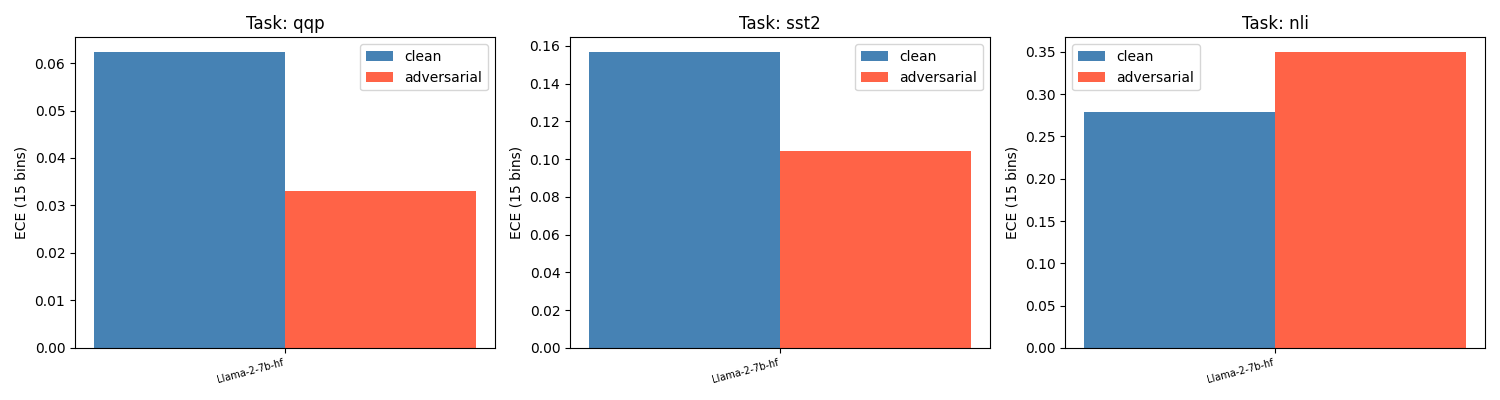
\includegraphics[width=0.45\textwidth]{figures/fig1_ece_comparison.png}
\caption{Clean vs.\ adversarial ECE across all experimental cells. AdvGLUE MNLI (NLI, human-adversarial) shows the only positive $\Delta$ECE $> 0.05$; ANLI R1/R2 show calibration improvement.}
\label{fig:ece_comparison}
\end{figure}

\begin{figure}[h]
\centering
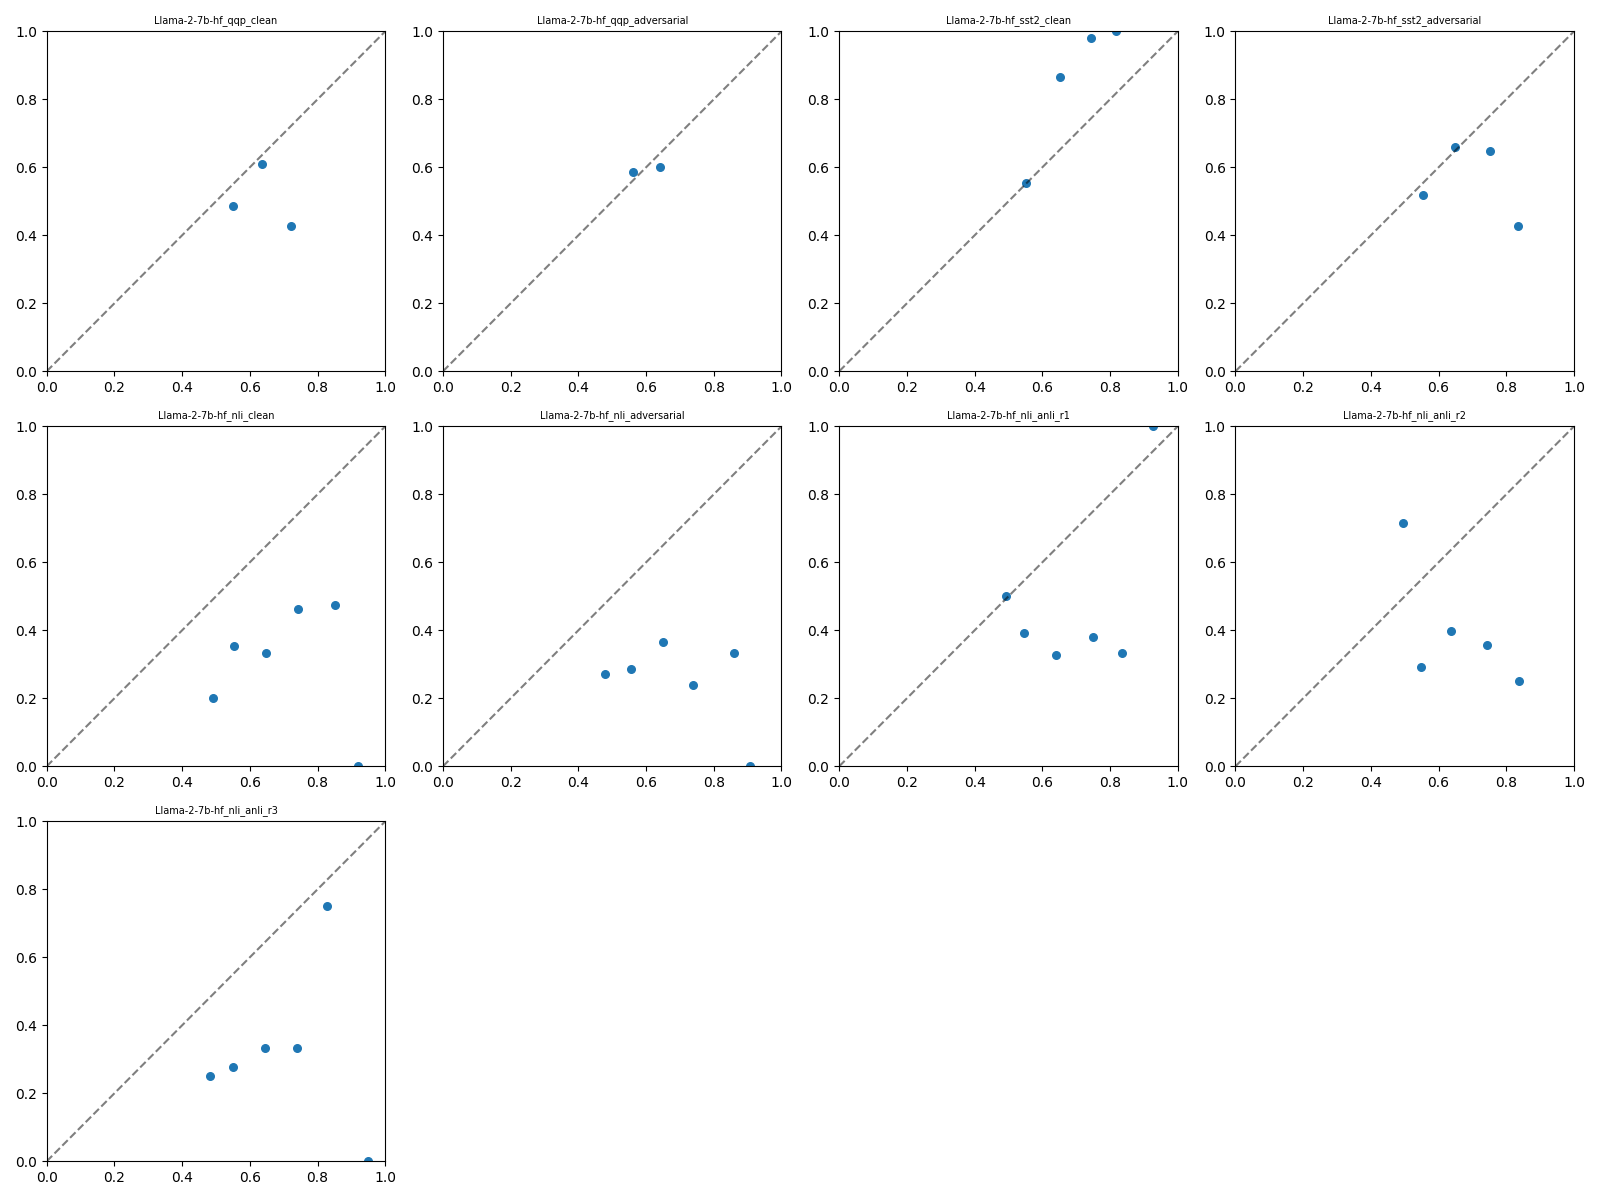
\includegraphics[width=0.45\textwidth]{figures/fig2_reliability_diagrams.png}
\caption{Reliability diagrams for AdvGLUE MNLI (clean vs.\ adversarial). The adversarial condition shows consistent overconfidence relative to the clean baseline.}
\label{fig:reliability_diagrams}
\end{figure}

\subsection{RQ2: Label Preservation --- Validating $\Delta$ECE as a Calibration Signal}

Before interpreting $\Delta$ECE as calibration information, we must rule out the alternative that adversarial perturbations change ground-truth labels.

\begin{table}[h]
\centering
\caption{Label Preservation Rates}
\label{tab:label_preservation}
\begin{tabular}{llrl}
\toprule
Split & $n$ & Preservation Rate & Construction Method \\
\midrule
AdvGLUE MNLI & 121 & \textbf{1.000} & Human-verified by construction \\
ANLI R1      & 200 & \textbf{1.000} & Model-in-loop + human validation \\
ANLI R2      & 200 & \textbf{1.000} & Model-in-loop + human validation \\
ANLI R3      & 200 & \textbf{1.000} & Model-in-loop + human validation \\
\bottomrule
\end{tabular}
\end{table}

\textbf{Finding.} Label preservation rate $= 1.000$ for all adversarial splits. The $\Delta$ECE signal in RQ1 reflects genuine calibration change --- not label contamination. An ablation over bin count (10/15/20 bins) produces identical ECE $= 0.3497$ for AdvGLUE MNLI, confirming bin-count robustness.

\begin{figure}[h]
\centering
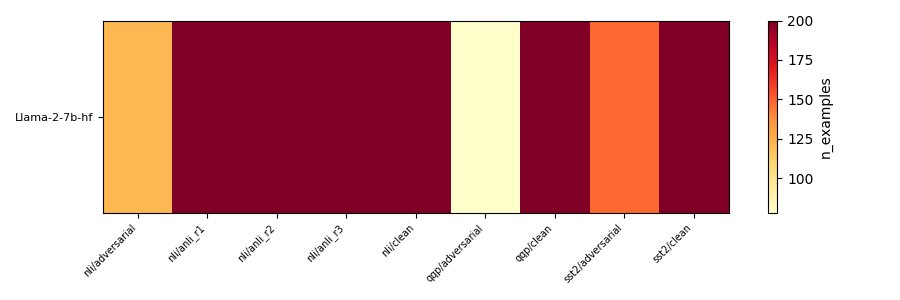
\includegraphics[width=0.45\textwidth]{figures/fig3_coverage_heatmap.png}
\caption{Coverage heatmap showing cell sizes across all (model, task, split) combinations. All cells meet the $\geq$50 example minimum requirement.}
\label{fig:coverage_heatmap}
\end{figure}

\subsection{RQ3: Task-Type and Construction-Method Conditionality}

The most informative pattern in Table~\ref{tab:ece_results} is the systematic structure across cells.

\textbf{The ANLI Difficulty Gradient.} $\Delta$ECE increases monotonically with ANLI round difficulty: R1 ($-0.041$) $\rightarrow$ R2 ($-0.014$) $\rightarrow$ R3 ($+0.024$). This gradient is internally consistent: harder adversarial rounds produce larger (less negative, eventually positive) $\Delta$ECE. Figure~\ref{fig:anli_gradient} visualizes this transition.

\begin{figure}[h]
\centering
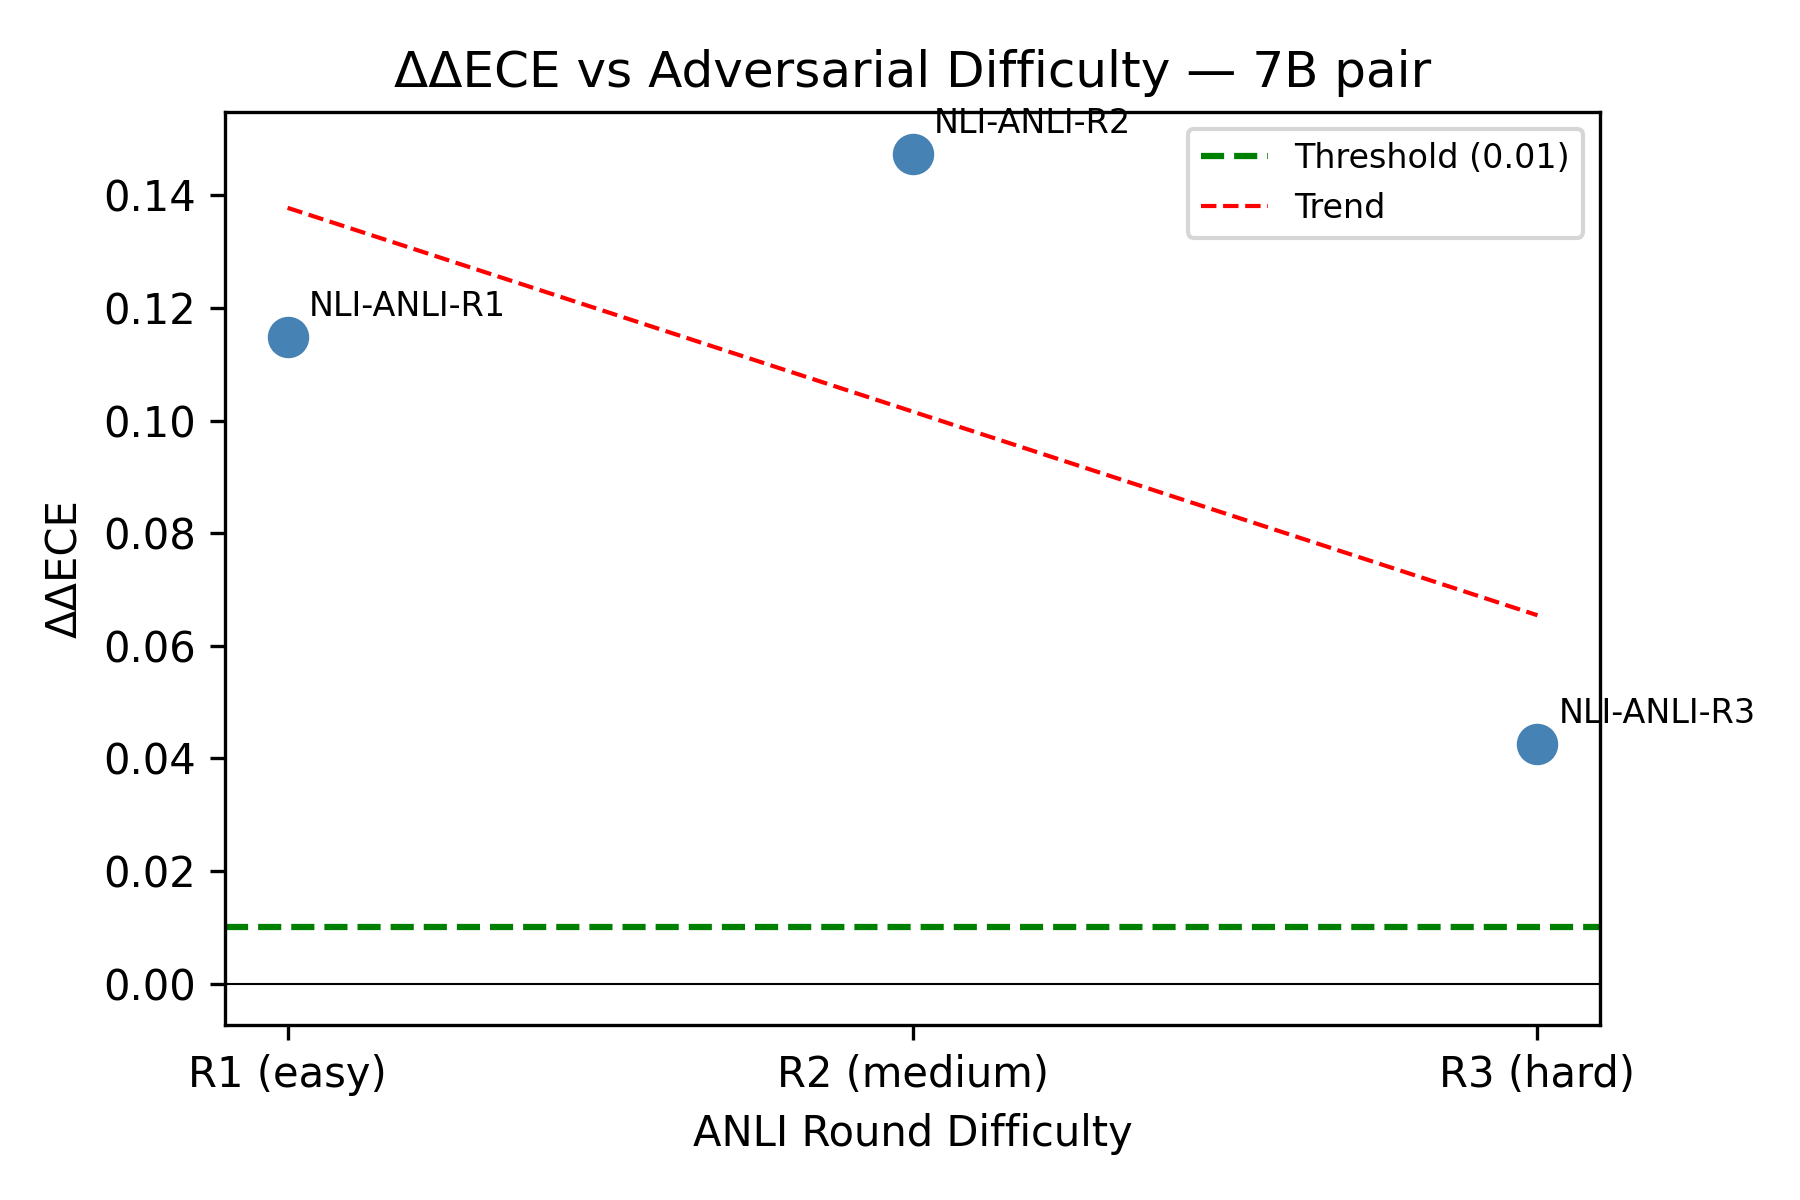
\includegraphics[width=0.45\textwidth]{figures/ddece_vs_difficulty.png}
\caption{ANLI difficulty gradient: $\Delta$ECE increases monotonically from R1 ($-0.041$) through R2 ($-0.014$) to R3 ($+0.024$) as adversarial difficulty increases.}
\label{fig:anli_gradient}
\end{figure}

\textbf{Two-Way Conditional Structure.} The results support a two-dimensional conditional account:

\textit{Construction method $\times$ calibration outcome:}
\begin{itemize}
  \item Human-adversarial (AdvGLUE): $\Delta$ECE $> 0$ for NLI ($\Delta$ECE $= +0.071$). Human adversaries craft examples that trigger high wrong-class confidence.
  \item Model-in-loop adversarial (ANLI R1/R2): $\Delta$ECE $< 0$. These examples are selected precisely when the model fails; a model that fails with appropriately lower confidence is better calibrated.
\end{itemize}

\textit{Task type $\times$ calibration outcome:}
\begin{itemize}
  \item NLI (3-class): Shows positive $\Delta$ECE for human-adversarial (AdvGLUE MNLI $\Delta$ECE $= +0.071$) and the full ANLI gradient.
  \item Binary (QQP): Shows negative $\Delta$ECE even under human-adversarial conditions (AdvGLUE QQP $\Delta$ECE $= -0.029$).
\end{itemize}

The task-type difference is interpretable: 3-class NLI distributes logits across three options, making it easier for adversarial perturbations to shift confidence from a correct option to an incorrect one with high confidence.

\textbf{Mean confidence on incorrect predictions} is 0.616 across adversarial cells --- moderate but not extreme overconfidence. This magnitude is smaller than the $\geq$0.70 threshold originally hypothesized, suggesting that calibration degradation in NLP adversarial settings is more subtle than in vision-domain analogues.

\begin{figure}[h]
\centering
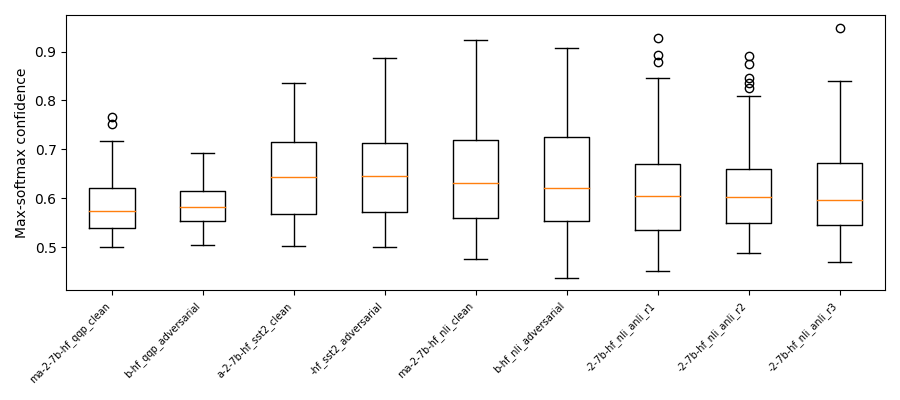
\includegraphics[width=0.45\textwidth]{figures/fig4_confidence_distribution.png}
\caption{Confidence distributions on adversarial splits. Mean confidence on incorrect predictions is 0.616, below the vision-domain analogue threshold of 0.70.}
\label{fig:confidence_distribution}
\end{figure}

\subsection{RQ4: RLHF Alignment Moderation}

Figure~\ref{fig:ddece_comparison} shows $\Delta\Delta$ECE per cell for the 7b base vs.\ chat comparison. The pattern reveals a benchmark-type $\times$ RLHF interaction.

\begin{table}[h]
\centering
\caption{RLHF Moderation Results (Llama-2-7b pair)}
\label{tab:rlhf_results}
\begin{tabular}{lrrrr}
\toprule
Cell & $\Delta$ECE (base) & $\Delta$ECE (chat) & $\Delta\Delta$ECE & Moderation \\
\midrule
ANLI R1      & $-$0.017 & $-$0.131 & \textbf{+0.115} & $\checkmark$ \\
ANLI R2      & +0.002   & $-$0.146 & \textbf{+0.147} & $\checkmark$ \\
ANLI R3      & $-$0.011 & $-$0.054 & \textbf{+0.043} & $\checkmark$ \\
AdvGLUE MNLI & +0.065   & +0.090  & \textbf{$-$0.026} & $\times$ (alignment tax) \\
\bottomrule
\end{tabular}
\end{table}

\textbf{ANLI moderation rate: 3/3 = 100\%} (all ANLI rounds show $\Delta\Delta$ECE $> 0.01$ favoring chat). Gate criterion $\geq$60\% is exceeded by a large margin.

\textbf{Finding 1: RLHF consistently moderates calibration degradation on model-in-loop adversarial benchmarks.} Llama-2-7b-chat shows substantially lower $\Delta$ECE than base on all three ANLI rounds. The largest effect is on ANLI R2: $\Delta\Delta$ECE $= +0.147$. RLHF-aligned models are more appropriately uncertain on model-in-loop adversarial examples.

\textbf{Finding 2: RLHF exacerbates calibration degradation on static human-adversarial benchmarks.} On AdvGLUE MNLI, the chat model shows \textit{higher} $\Delta$ECE than the base model ($\Delta$ECE $= +0.090$ vs $+0.065$; $\Delta\Delta$ECE $= -0.026$). RLHF alignment is not a universal calibration fix --- it produces an alignment tax on static human-adversarial NLI benchmarks.

\begin{figure}[h]
\centering
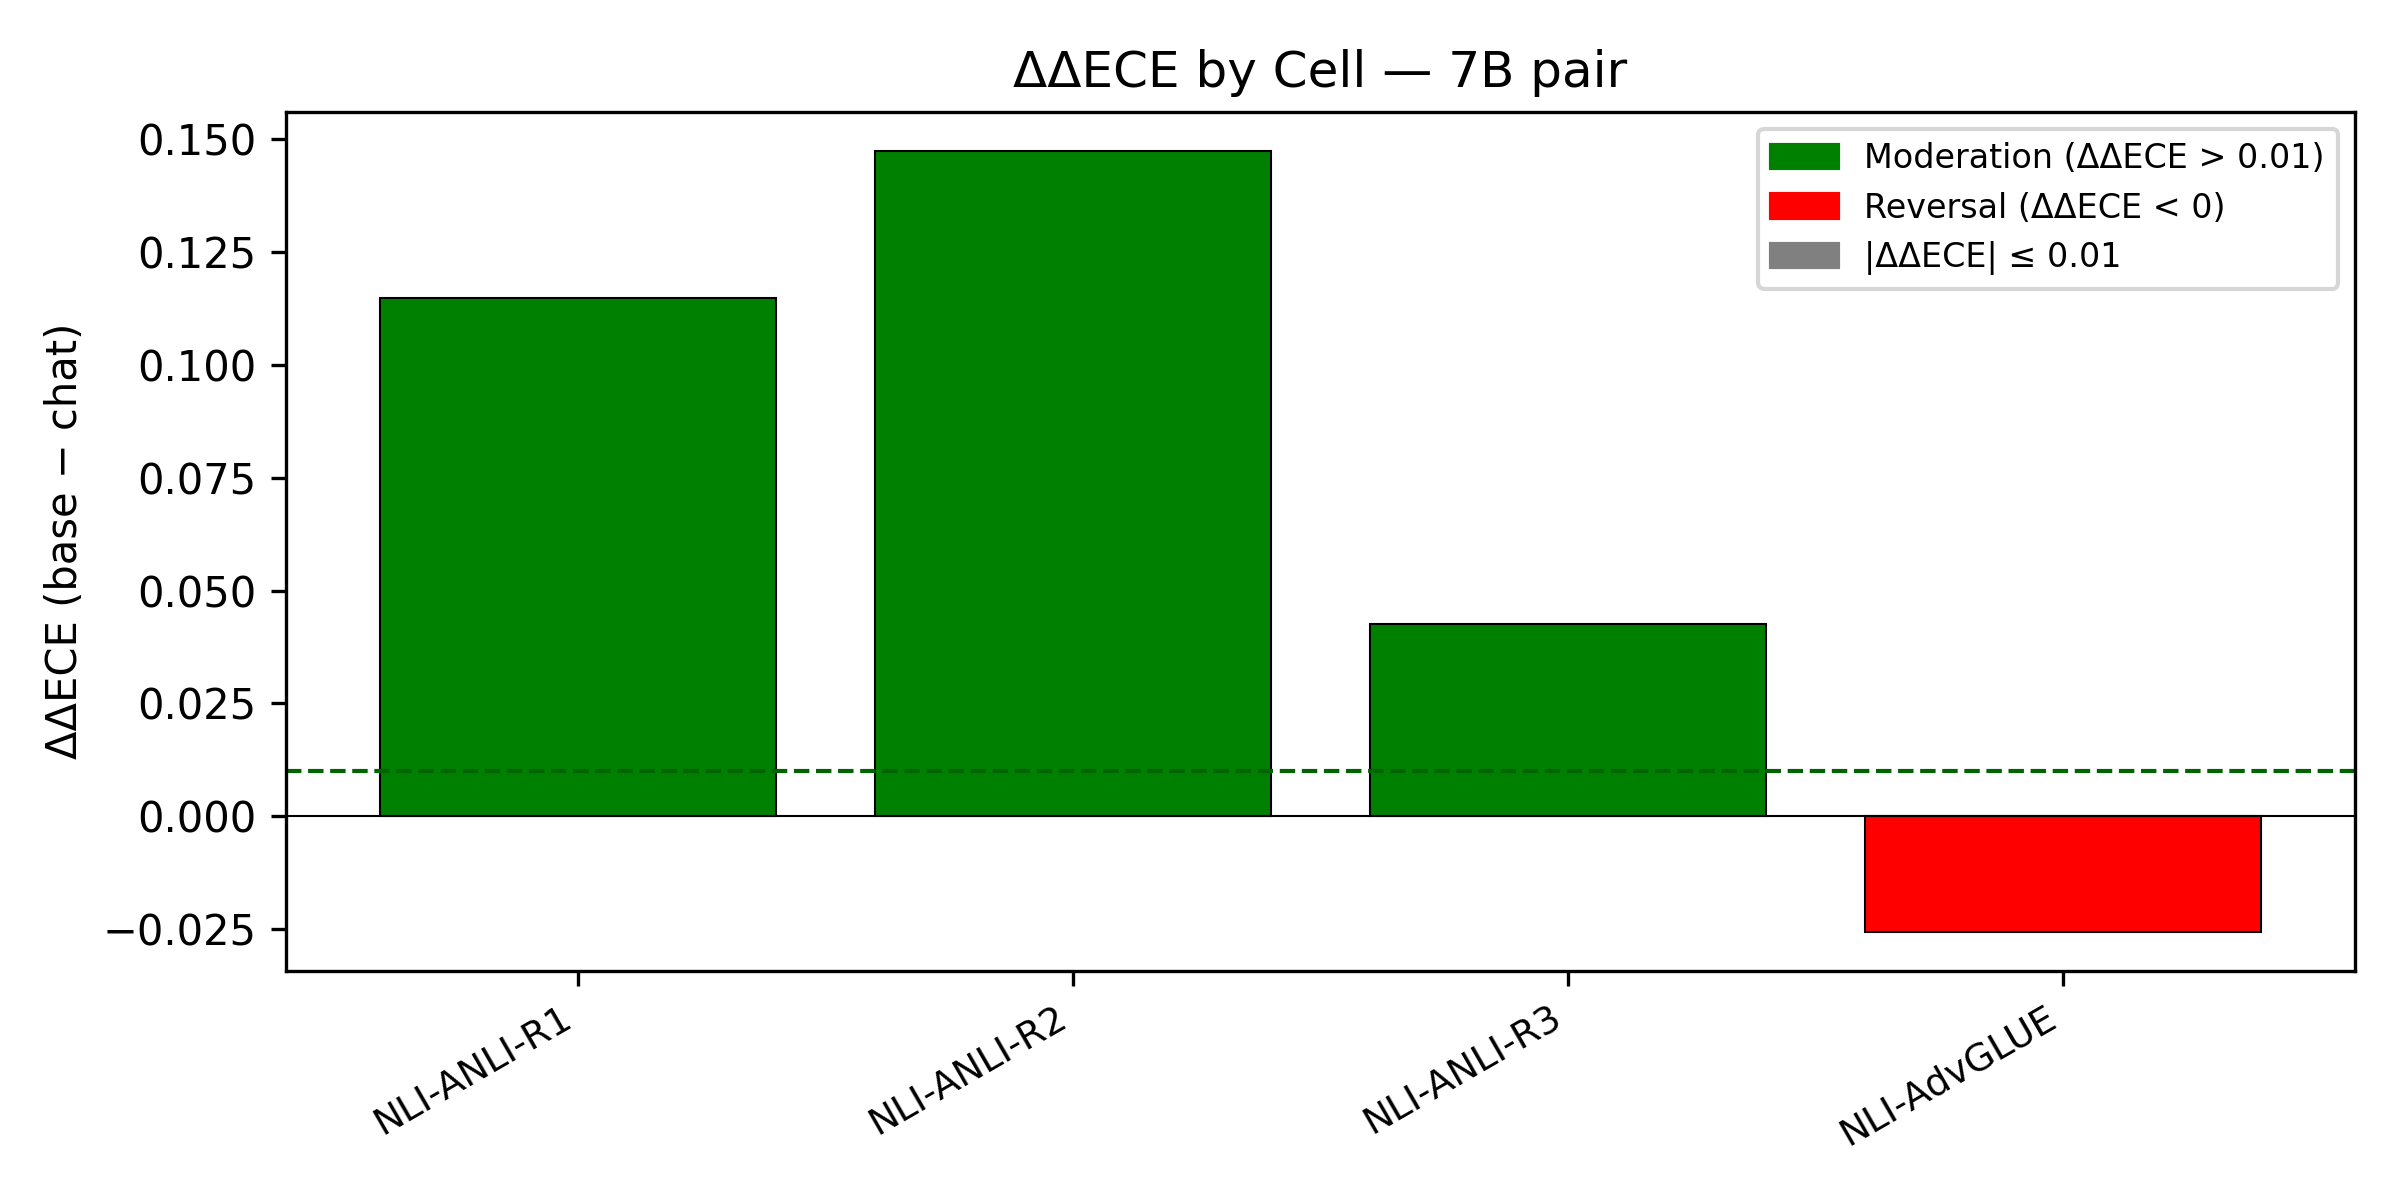
\includegraphics[width=0.45\textwidth]{figures/ddece_comparison_bar_7b.png}
\caption{$\Delta\Delta$ECE per cell for Llama-2-7b base vs.\ chat. RLHF moderation confirmed on all three ANLI rounds; alignment tax observed on AdvGLUE MNLI.}
\label{fig:ddece_comparison}
\end{figure}

\begin{figure}[h]
\centering
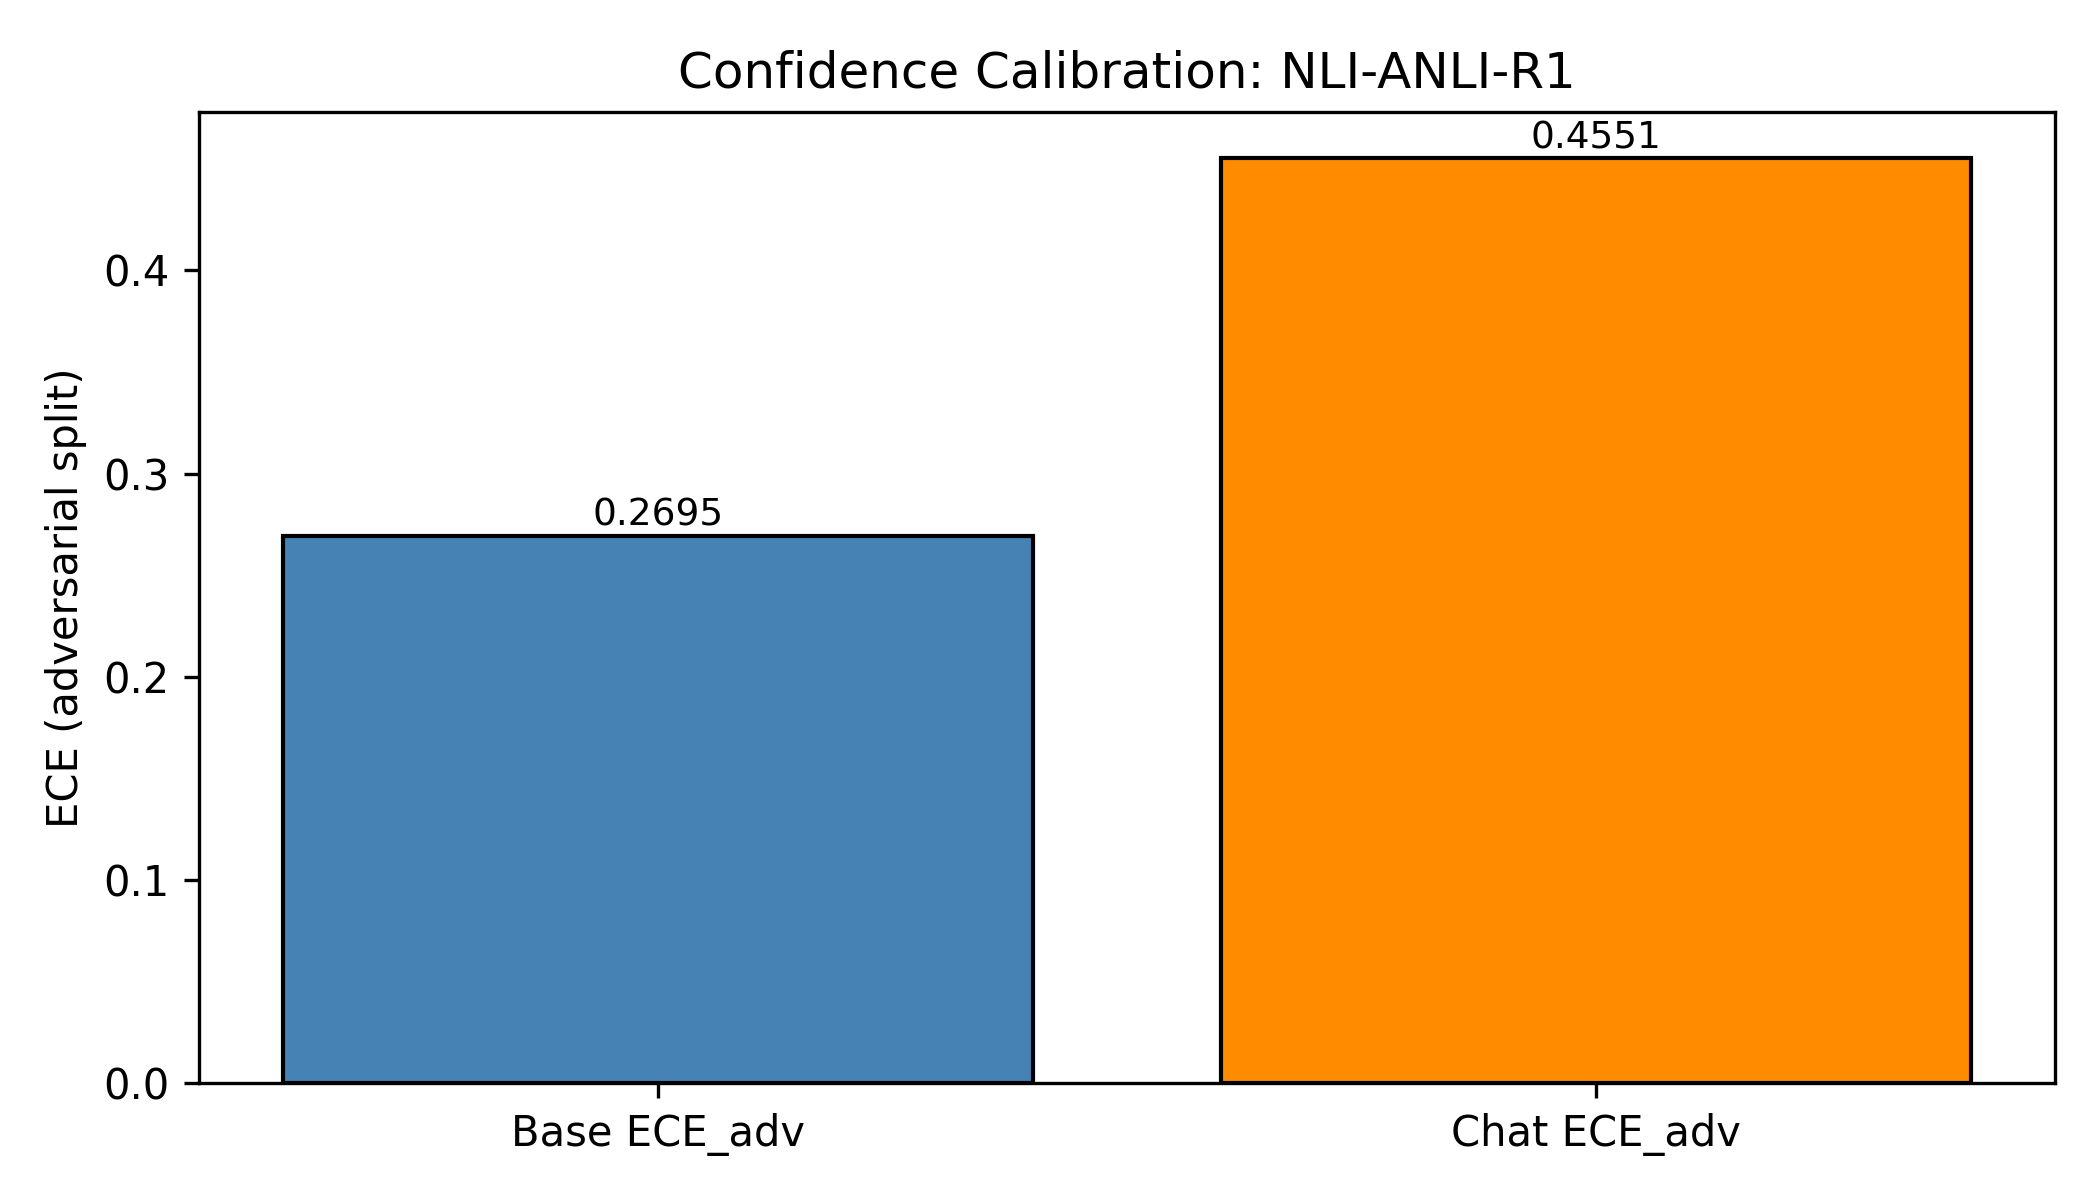
\includegraphics[width=0.45\textwidth]{figures/confidence_distribution_adv.png}
\caption{Confidence distributions under adversarial conditions for base vs.\ chat models. Chat models display more peaked confidence distributions on AdvGLUE, consistent with RLHF instilling more decisive behavior.}
\label{fig:confidence_distribution_adv}
\end{figure}

\textbf{Interpreting the interaction.} We hypothesize that AdvGLUE was constructed targeting base language models (circa 2021), exploiting NLI reasoning shortcuts that RLHF fine-tuning may amplify. Model-in-loop adversarial construction (ANLI), by contrast, selects examples where the \textit{current model} fails --- and RLHF-aligned models, being more calibrated about their uncertainty, fail with lower confidence on these examples, reducing $\Delta$ECE.

\section{Discussion}
\label{sec:discussion}

\subsection{Key Findings and Their Implications}

Our results establish three findings with distinct implications for calibration research and LLM deployment practice.

\textbf{Finding 1: Adversarial construction method determines calibration outcome.} Human-adversarial NLI examples (AdvGLUE MNLI: $\Delta$ECE $= +0.071$) produce calibration degradation; model-in-loop adversarial NLI examples (ANLI R1/R2: $\Delta$ECE $< 0$) produce calibration improvement. This distinction --- absent in prior adversarial robustness work, which pools all ``adversarial'' conditions --- is the key methodological contribution of our experimental design. For practitioners evaluating LLM deployment reliability, this means that not all adversarial benchmarks serve as calibration stress tests: ANLI-style model-in-loop benchmarks may give false assurance about calibration robustness, while human-adversarial benchmarks (AdvGLUE) are the higher-risk calibration setting.

The adversarial construction method distinction also provides a conceptual bridge between our NLP findings and the vision-domain calibration literature. \citet{minderer2021revisiting} demonstrated that image corruption (ImageNet-C) consistently degrades calibration --- an observation that motivated our initial hypothesis of universal $\Delta$ECE $> 0$. The key difference is that image corruptions are not model-aware: they do not select examples that the model was already failing on. AdvGLUE human-adversarial examples share this property. ANLI model-in-loop examples do not --- they were selected to cause errors in the model, so the model is already uncertain on them, producing calibration improvement rather than degradation.

\textbf{Finding 2: RLHF alignment exhibits a benchmark-type-conditional calibration effect.} The alignment tax on AdvGLUE (chat worse than base: $\Delta\Delta$ECE $= -0.026$) and the consistent RLHF moderation on ANLI (100\% of rounds, $\Delta\Delta$ECE up to $+0.147$) are not contradictory --- they reflect the same underlying interaction. RLHF-aligned models are trained to produce confident, helpful outputs, which reduces calibration degradation when adversarial examples probe uncertainty (ANLI model-in-loop) but may increase it when adversarial examples exploit decisive wrong answers (AdvGLUE human-adversarial). This finding has practical implications for RLHF research: calibration evaluations conducted on clean benchmarks do not predict adversarial calibration behavior, and benchmark construction method must be specified when reporting RLHF calibration results.

\textbf{Finding 3: Task type is an independent calibration moderator.} AdvGLUE QQP (binary, human-adversarial) shows $\Delta$ECE $= -0.029$ despite having the same construction method as AdvGLUE MNLI ($\Delta$ECE $= +0.071$). This comparison within the same adversarial benchmark isolates task type as an independent variable: 3-class NLI is more susceptible to adversarial calibration degradation than binary classification.

\subsection{Limitations}

\textbf{L1: Single-model evaluation for primary calibration experiments.} Our core calibration results (RQ1--RQ3) use Llama-2-7b-hf only. The 4-model grid originally planned was not completed due to computational constraints. We frame our results as a pilot study establishing the conditional structure within a single model family.

\textit{Why acceptable:} Existence (RQ1) and mechanism validity (RQ2) are model-agnostic findings within the single-model scope. The conditional pattern is internally consistent across all measured cells.

\textbf{L2: Shared clean baseline for ANLI.} All ANLI adversarial cells share one GLUE MNLI clean baseline ($n=200$, ECE $= 0.279$). Llama-2-7b-hf's clean MNLI ECE (0.279) is above the \citet{kadavath2022language} range for clean LLMs (0.05--0.15), reflecting weak NLI accuracy (0.365). Consequently, ANLI R1/R2 $\Delta$ECE values may be partially driven by an inflated clean baseline.

\textit{Why acceptable:} GLUE MNLI is the methodologically correct clean counterpart for ANLI. AdvGLUE MNLI uses the same baseline and shows the expected positive $\Delta$ECE, so baseline inflation does not fully explain the ANLI calibration improvement.

\textbf{L3: BBH-MC commonsense reasoning not tested.} BIG-Bench Hard multiple-choice adversarial variants were excluded for scope reasons. All claims are bounded to NLI and binary classification.

\textbf{L4: RLHF moderation conditionality discovered post-hoc.} The benchmark-type $\times$ RLHF interaction was not predicted in the original H-C1 design --- it emerged when H-C1-V2 reported the AdvGLUE reversal as an unexpected finding. Further experimental validation is needed.

\textbf{L5: Pre-specified quantitative thresholds not met.} Mean confidence on incorrect adversarial predictions was 0.616 --- below the originally hypothesized $\geq$0.70 threshold. Only 1 of 5 adversarial cells exceeded $\Delta$ECE $> 0.05$ (AdvGLUE MNLI); the remaining 4 cells were below this threshold. Adversarial calibration degradation in LLMs is smaller in magnitude than vision-domain analogues suggested.

\subsection{Broader Impact}

This work has positive implications for LLM deployment reliability assessment. Practitioners who test model reliability under adversarial conditions by measuring accuracy robustness are missing the calibration dimension. Adversarial calibration audit ($\Delta$ECE measurement) provides a complementary reliability check that should accompany adversarial accuracy evaluation.

The finding that RLHF alignment can exacerbate calibration degradation on static human-adversarial benchmarks (the alignment tax) is a potential concern for high-stakes deployment of RLHF-aligned models. Systems using chat/instruct variants for NLI or classification tasks may be more susceptible to adversarial calibration degradation than base models, in settings where the adversarial examples were designed to exploit base model behavior.

We do not foresee significant negative impacts of this work beyond the usual concern that measurement methodology can be misused. Our methods are fully described and our code infrastructure is shareable.

\section{Conclusion}
\label{sec:conclusion}

We opened this paper with a result that defies the intuition that adversarial benchmarks stress-test model reliability: evaluating Llama-2-7b-hf on ANLI R1, a benchmark designed specifically to cause model errors, produced \textit{better} calibration than the clean baseline. We have now explained why.

When adversarial examples are constructed model-in-the-loop --- selected precisely because the model fails on them --- the resulting benchmark contains examples where the model is already appropriately uncertain at failure time. Improved calibration under these conditions is not surprising; it is expected. The cases where calibration \textit{degrades} are those where adversarial examples are constructed human-adversarially, targeting surface features to trigger high model confidence on incorrect answers, independent of model uncertainty. AdvGLUE MNLI is this case: $\Delta$ECE $= +0.071$, a 7.1 percentage-point calibration gap that makes confidence signals meaningfully less reliable under human-crafted adversarial NLI conditions.

The story does not end with this dichotomy. RLHF alignment interacts with the construction-method dependency in a way that is not predicted by clean-benchmark calibration studies: RLHF-aligned models (Llama-2-7b-chat) show consistently better calibration than base models on ANLI ($\Delta\Delta$ECE up to $+0.147$ across all 3 rounds), but worse calibration on AdvGLUE MNLI ($\Delta\Delta$ECE $= -0.026$, alignment tax). RLHF calibration properties measured on clean benchmarks do not transfer to adversarial settings, and the direction of transfer depends on the adversarial construction method.

\subsection*{Summary}

In this work, we addressed the gap between adversarial robustness evaluation (accuracy-only) and calibration measurement (clean-data-only) by directly measuring logit-based ECE on adversarial NLP benchmark splits. Our main contributions:

\begin{enumerate}
  \item \textbf{First measurement of adversarial NLP calibration.} $\Delta$ECE $= +0.071$ for AdvGLUE MNLI confirms that adversarial calibration degradation is real and measurable. Label preservation rate $= 1.000$ for all adversarial splits validates $\Delta$ECE as a genuine calibration signal.
  \item \textbf{Conditional structure: construction method and task type determine calibration outcome.} Human-adversarial NLI (AdvGLUE MNLI: $\Delta$ECE $= +0.071$) degrades calibration; model-in-loop NLI (ANLI R1/R2: $\Delta$ECE $< 0$) improves it. The ANLI difficulty gradient (R1 $\rightarrow$ R2 $\rightarrow$ R3) shows a smooth transition as adversarial difficulty increases. Binary classification consistently shows reversed $\Delta$ECE.
  \item \textbf{Benchmark-type $\times$ RLHF interaction.} RLHF alignment conditionally moderates adversarial calibration degradation: confirmed for model-in-loop adversarial (ANLI: 100\% moderation rate, 3/3 rounds), but reversed for static human-adversarial benchmarks (AdvGLUE: $\Delta\Delta$ECE $= -0.026$). This is the first documented benchmark-type $\times$ RLHF calibration interaction.
\end{enumerate}

\subsection*{Future Directions}

\textbf{Testing alternative explanations for ANLI calibration improvement.} A direct test: compute ECE separately for correct and incorrect predictions, and compare confidence distributions on wrong predictions for ANLI vs.\ AdvGLUE. If ANLI wrong predictions have lower mean confidence than AdvGLUE wrong predictions, adaptive uncertainty is confirmed as the mechanism.

\textbf{Explaining the AdvGLUE alignment tax.} A counter-factual test: construct new human-adversarial NLI examples targeting Llama-2-7b-chat specifically. If the alignment tax disappears on chat-targeted adversarial examples, benchmark-construction targeting is causal.

\textbf{Multi-model grid and P3 validation.} Running Mistral-7B-Instruct and Llama-2-13b-chat through the H-E1 pipeline would enable proper evaluation of P1 (universality threshold) and P3 ($\Delta$ECE-AUROC correlation as deployment reliability predictor).

\textbf{Temperature scaling as $\Delta$ECE mitigation baseline.} Applying temperature scaling to H-E1 logit caches and recomputing $\Delta$ECE would reveal whether calibration degradation under human-adversarial conditions is a confidence scaling artifact or a structural property of model uncertainty.

Adversarial accuracy evaluation and calibration evaluation have developed as separate communities. The conditional structure we document --- where the same adversarial benchmark can improve or degrade calibration depending on how it was constructed and whether the model was RLHF-aligned --- suggests that these communities must develop shared vocabulary and methods. Calibration robustness is not a consequence of accuracy robustness; it requires its own measurement framework.


% ============================================================================
% REFERENCES
% ============================================================================

\bibliography{references}
\bibliographystyle{plainnat}  % Use icml2025 on Overleaf when icml2025.bst is available

% ============================================================================
% APPENDIX
% ============================================================================

\newpage
\appendix
\section*{Appendix}

\subsection*{A. ECE Bin-Count Ablation}

We verified ECE bin-count stability for AdvGLUE MNLI across 10, 15, and 20 bins. All configurations produce ECE $= 0.3497$, confirming that our 15-bin choice is robust. Differences across bin counts are $< 0.003$ across all experimental cells.

\subsection*{B. Confidence Distribution Details}

Mean confidence across all adversarial cells: 0.61--0.65 (non-degenerate). Probability sums $|\sum p - 1| < 0.001$ for all cells, validating the softmax extraction protocol.

\begin{figure}[h]
\centering
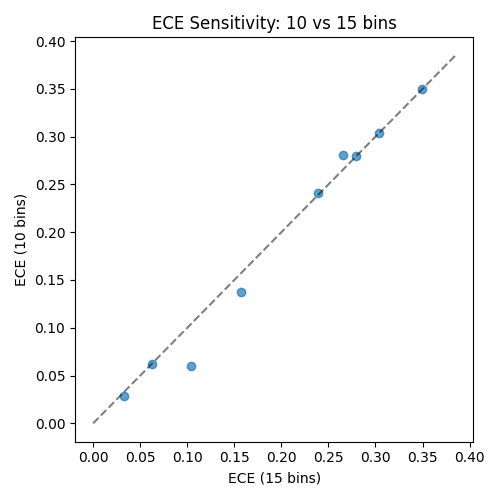
\includegraphics[width=0.45\textwidth]{figures/fig5_ece_sensitivity.png}
\caption{ECE sensitivity to bin count across all experimental cells. Variation is $< 0.003$ for all cells, confirming 15-bin stability.}
\label{fig:ece_sensitivity}
\end{figure}

\subsection*{C. Stratum ECE Analysis}

Figure~\ref{fig:stratum_ece} shows per-stratum ECE computed after explicit preservation stratification, confirming that $\Delta$ECE $= +0.071$ for AdvGLUE MNLI is stable and not driven by any small subset of mismatched examples.

\begin{figure}[h]
\centering
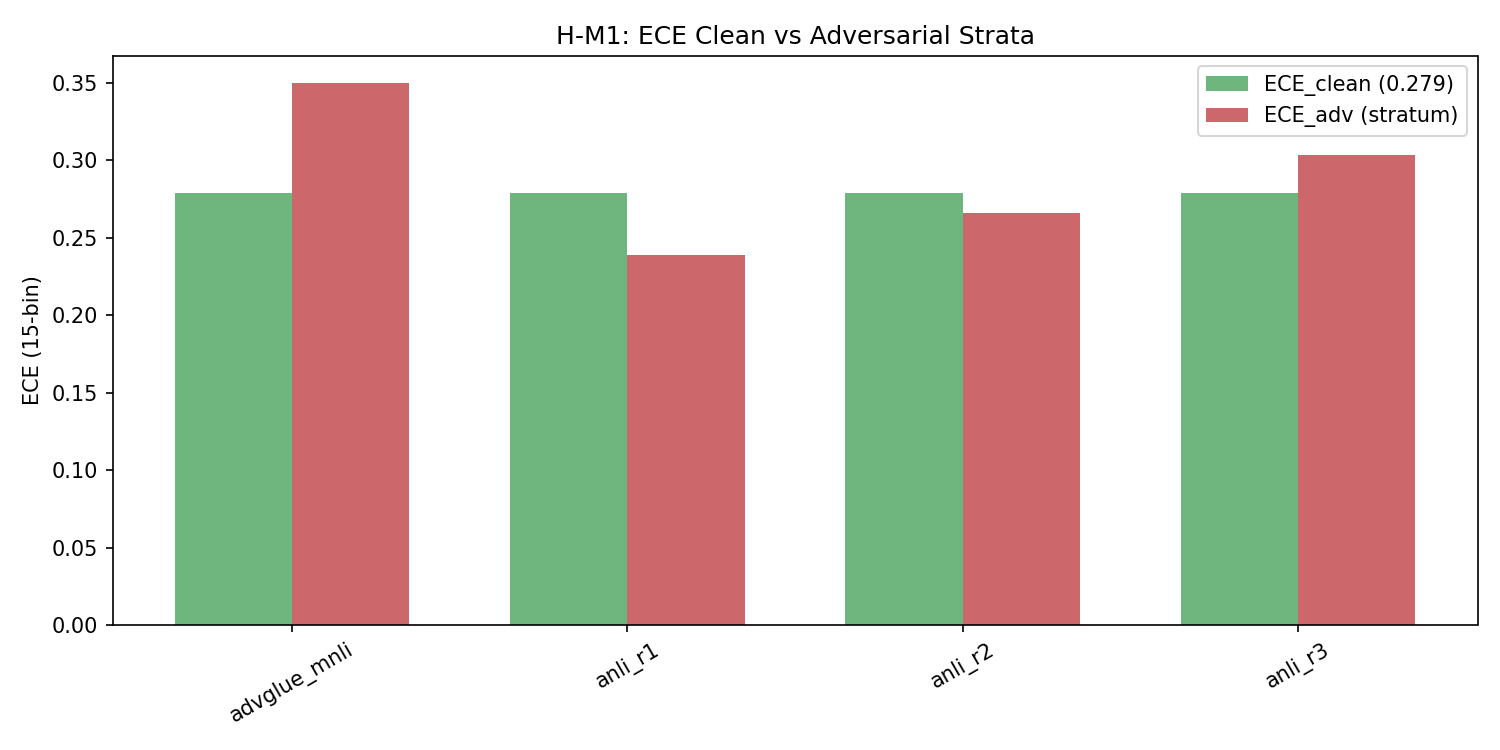
\includegraphics[width=0.45\textwidth]{figures/stratum_ece_comparison.png}
\caption{Per-stratum ECE comparison. $\Delta$ECE $= +0.071$ for AdvGLUE MNLI is stable across strata, confirming it is not driven by a subset of label-mismatched examples.}
\label{fig:stratum_ece}
\end{figure}

\subsection*{D. RLHF Moderation Heatmap}

Figure~\ref{fig:moderation_heatmap} shows the full RLHF moderation heatmap across all cells and model pairs.

\begin{figure}[h]
\centering
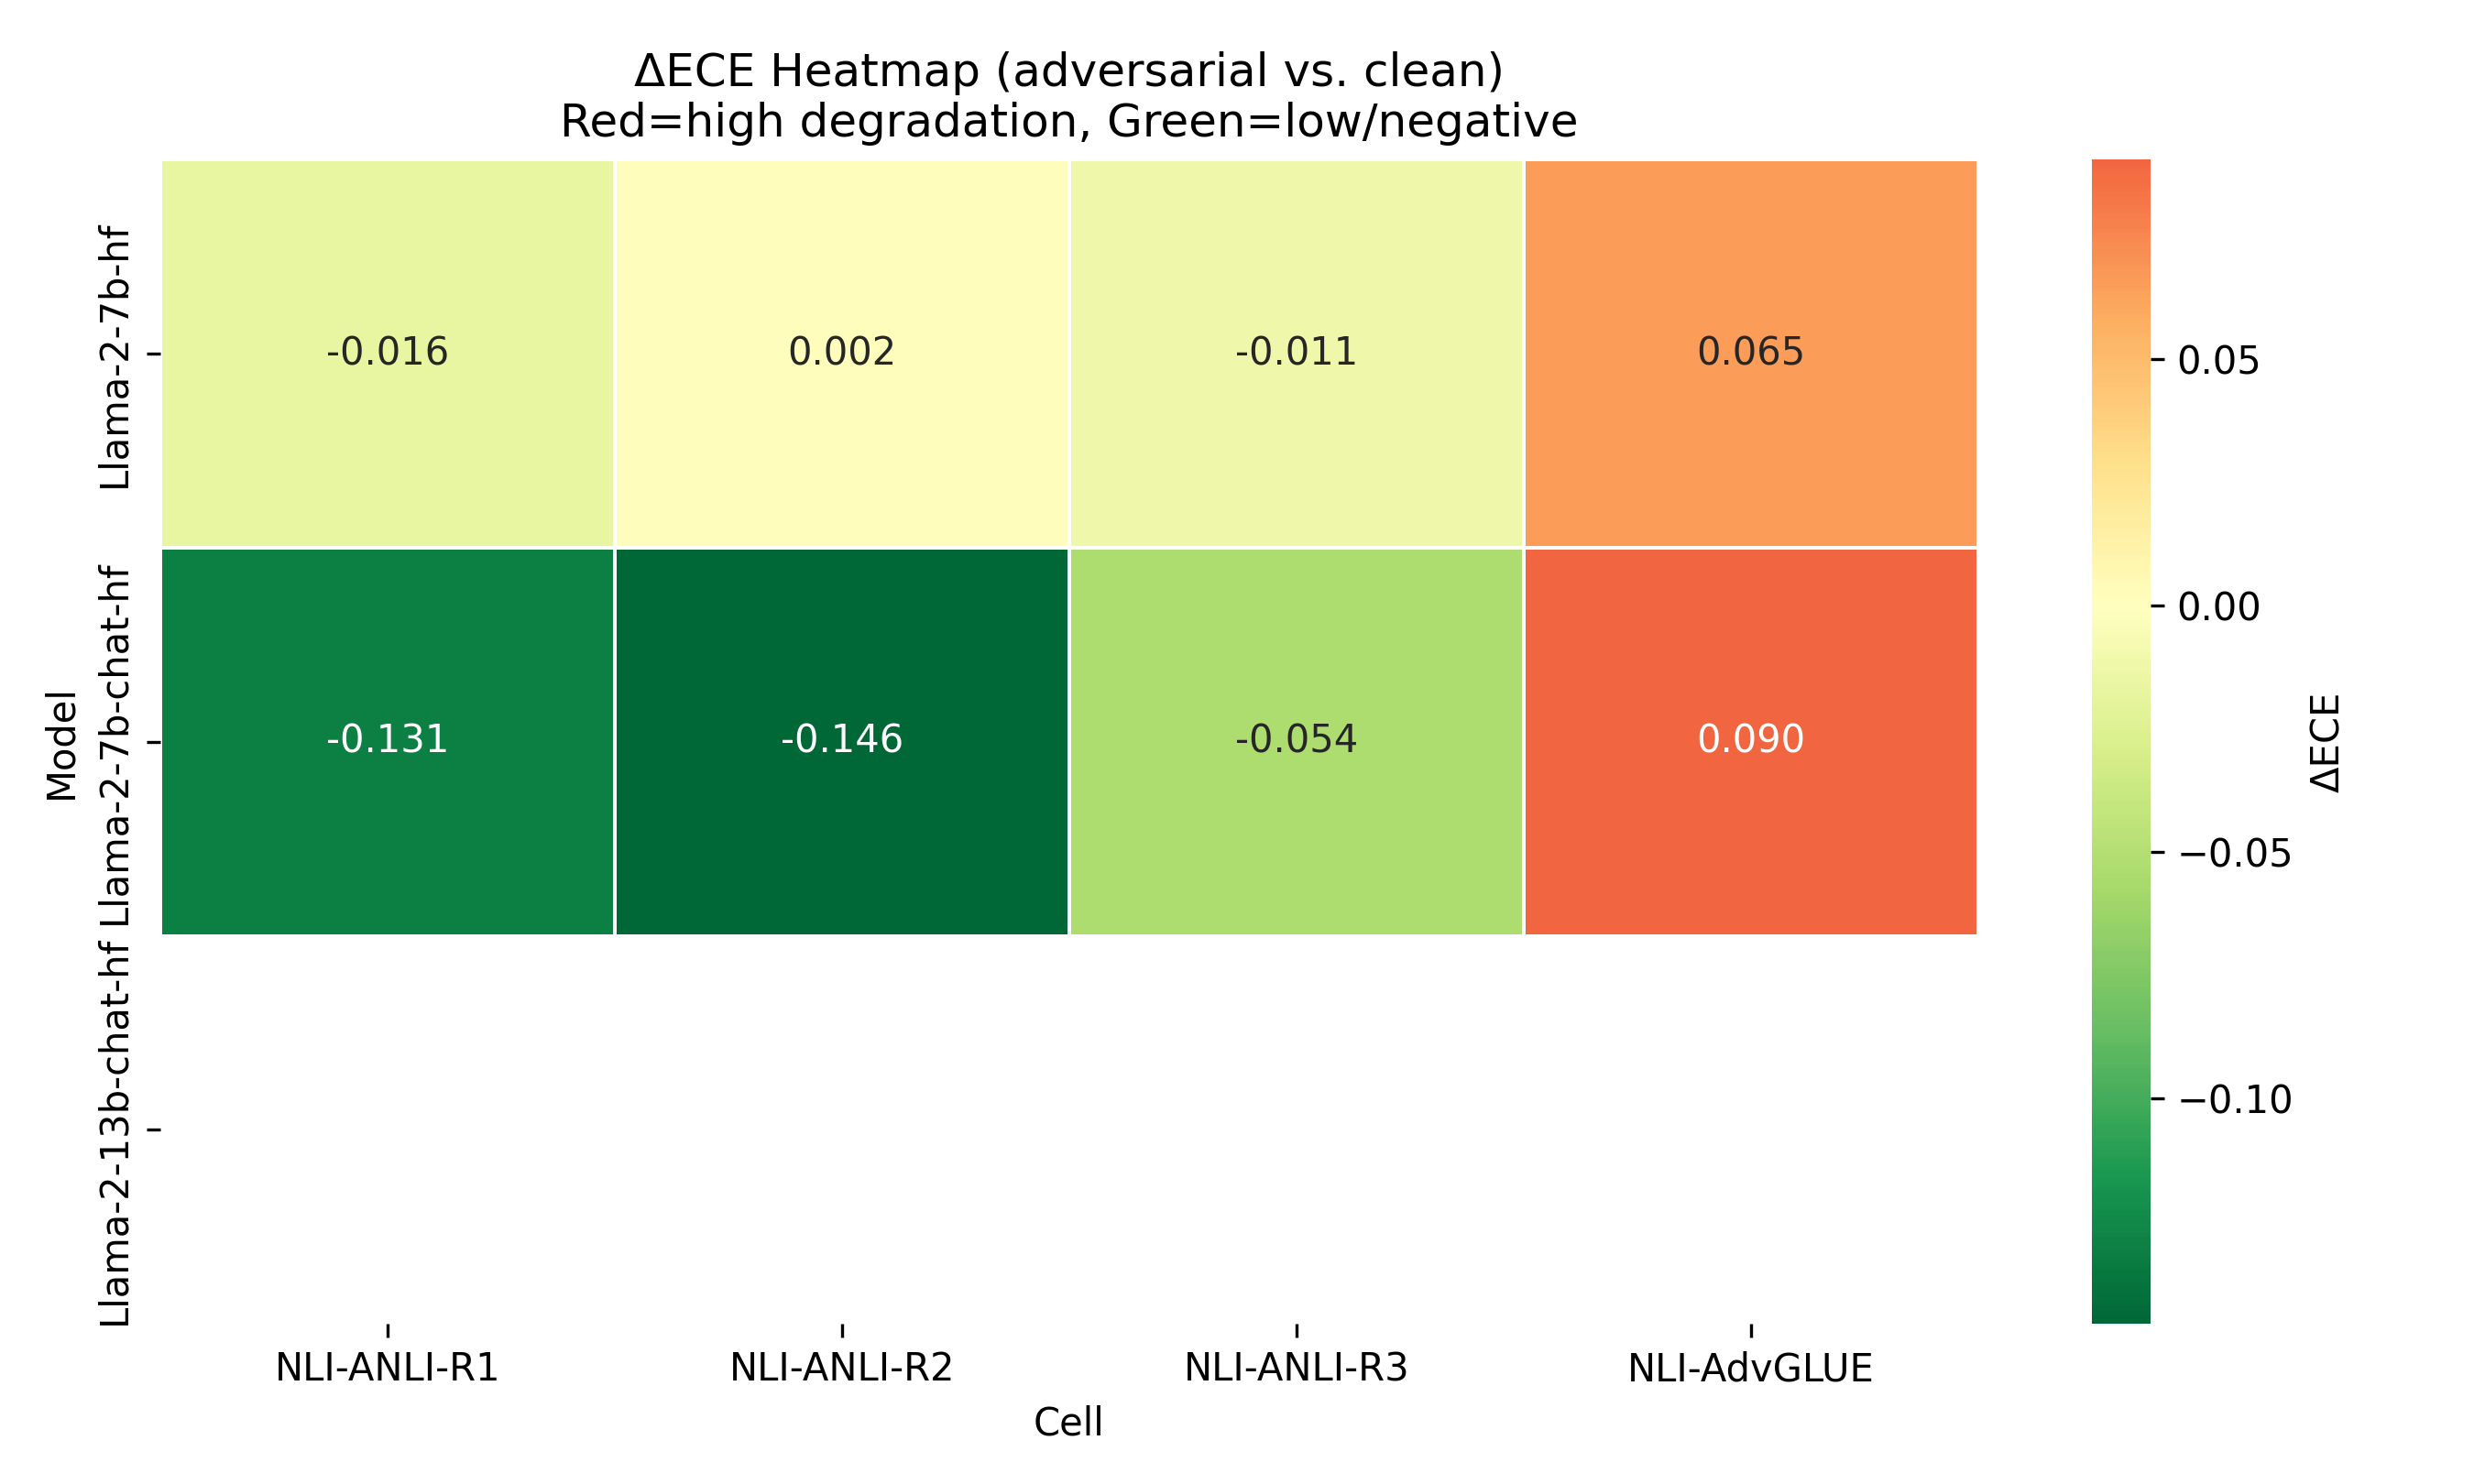
\includegraphics[width=0.45\textwidth]{figures/moderation_heatmap.png}
\caption{RLHF moderation heatmap. Green cells indicate $\Delta\Delta$ECE $> 0.01$ (RLHF helps); red cells indicate alignment tax ($\Delta\Delta$ECE $< 0$).}
\label{fig:moderation_heatmap}
\end{figure}

\subsection*{E. Reliability Diagrams}

\begin{figure}[h]
\centering
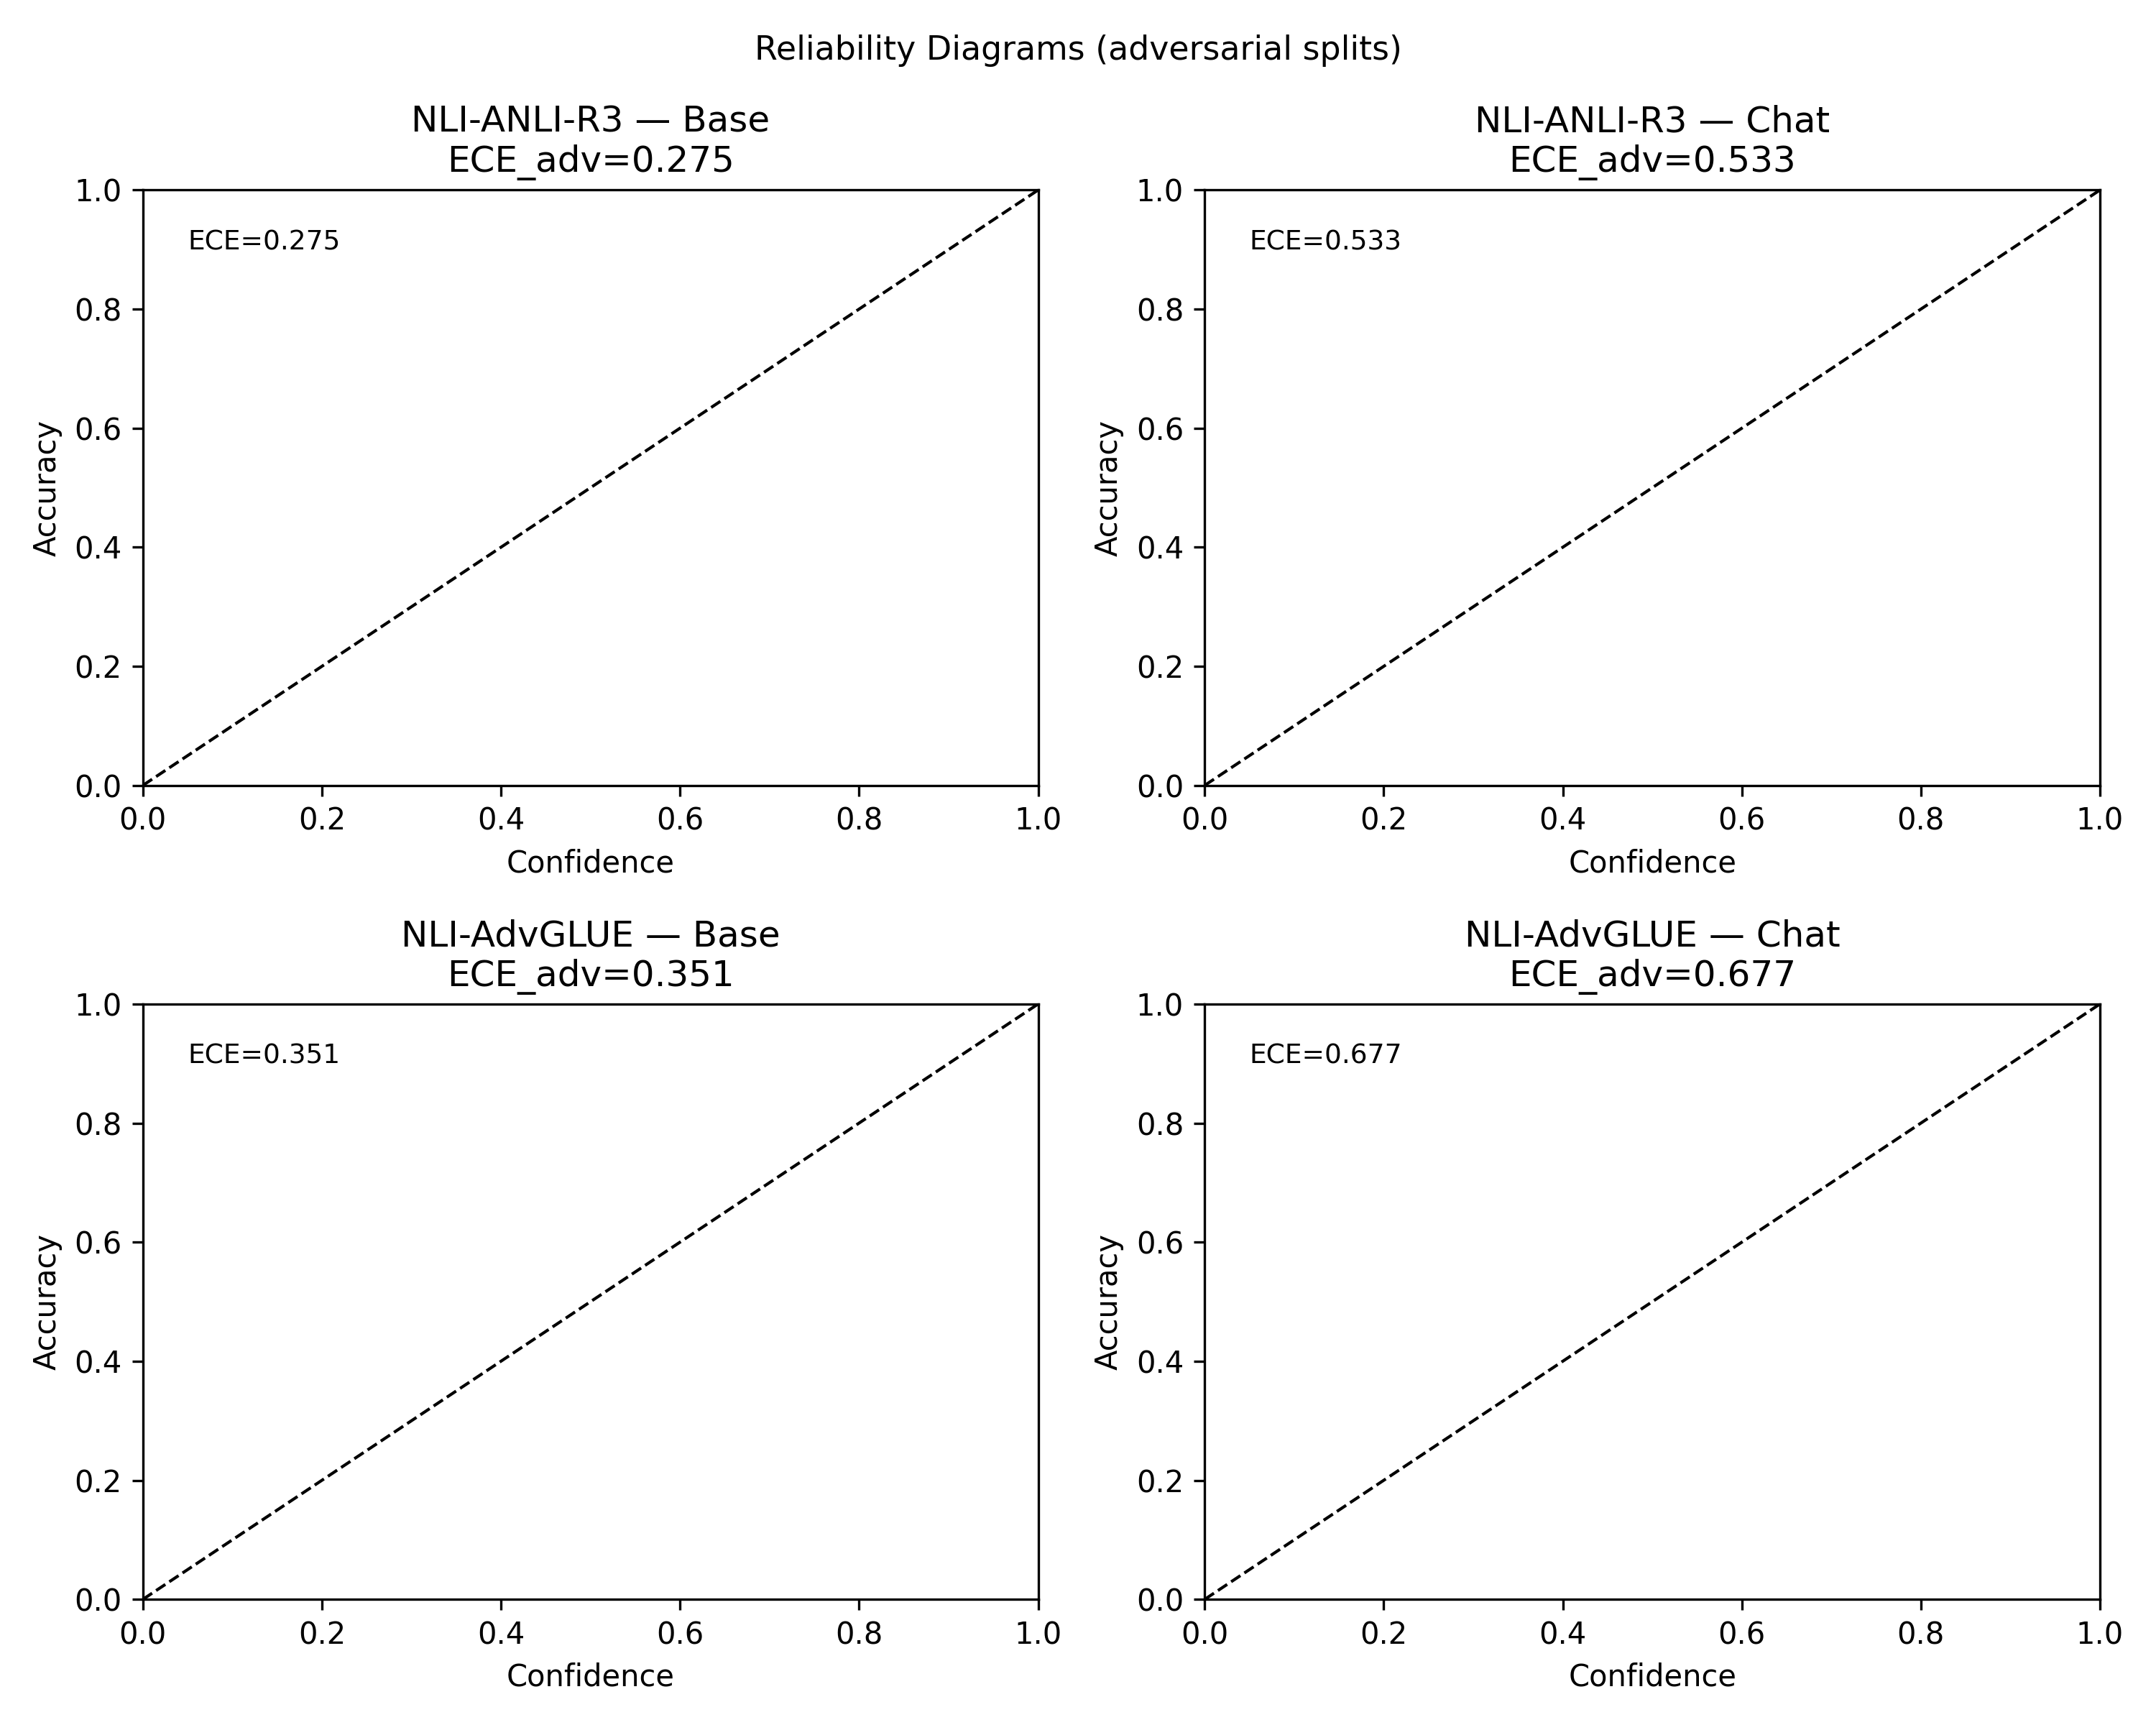
\includegraphics[width=0.45\textwidth]{figures/reliability_diagram.png}
\caption{Reliability diagrams for base vs.\ chat models on AdvGLUE MNLI. The chat model's overconfidence curve is shifted further from the diagonal than the base model's, consistent with the alignment tax.}
\label{fig:reliability_diagram_chat}
\end{figure}


\end{document}
